\documentclass[12pt ,letterpaper]{article}
\usepackage{amsmath}
\usepackage[utf8]{inputenc}
\usepackage{amsfonts}
\usepackage{amssymb}
\usepackage{graphicx}
\usepackage[T1]{fontenc}
%\usepackage[ngerman]{babel}
\usepackage{caption}
\usepackage{refstyle}
\usepackage[left=2cm, right=2cm, top=2cm, bottom=2cm]{geometry}
\usepackage[onehalfspacing]{setspace}
\usepackage{listings} 
\usepackage{tcolorbox}
\usepackage{subfig}
\usepackage{url}

\lstset{language=Java} 
 
\title{Edwards Biotope - Interdiszipliänres Projekt II - Abschlussbericht}
\date{01.08.2019}

\begin{document}
\begin{onehalfspace}
\maketitle
\tableofcontents
\pagebreak
\section{Abstract}
\section{Einleitung}
\pagebreak
\section{Roadmap}
\begin{longtable}{|p{8cm}|p{10cm}|}
\hline
\textbf{Organisation} &  \\ \hline
Planungsgremium & Manuela Mosandl \\ \hline
Werbeplakat und technisches Plakat & Robert Sabo \\ \hline
Projektpräsentation und Demo & Robert Sabo, Sebastian Beck, Gabriel Veiz, Pia Korndörfer, Felix Baumgarten \\ \hline
Erstellung Latex-Template und Umsetzung des Berichts in Latex & Sebastian Beck \\ \hline
\textbf{Game Design} &  \\ \hline
Fokus auf Stellungsspiel & Felix Baumgarten, Robert Sabo \\ \hline
Die Spielmechanik der Strömung & Robert Sabo, Felix Baumgarten \\ \hline
\textbf{Grafik- und Sounddesign} & \\ \hline
Produktion: Musik- und Soundeffekte & \\ \hline
Produktion Video: After Effects Tutorials & Cigdem Bozyigit \\ \hline
Produktion Video: Logo animieren & Cigdem Bozyigit \\ \hline
Produktion Video: Ideenfindung & Alle \\ \hline
Produktion Video: Projekt Video Intro & Manuela Mosandl \\ \hline
Produktion Video: Storyboard & Pamela Schättin, Manuela Mosandl, Gabriel Veiz \\ \hline
Produktion Video: Logo Animation für den Trailer & Pia Korndörfer, Robert Sabo \\ \hline
Produktion Video: Kompression des Trailers & Pia Korndörfer, Robert Sabo \\ \hline
Produktion Video: Animation Spielfeld & Gabriel Veiz \\ \hline
Produktion Musik und Sound & Philadelphia Gaus \\ \hline
Illustration: Lichtgebung und Schattierung & Manuela Mosandl \\ \hline
Illustration: Karten kolorieren & Pia Korndörfer \\ \hline
Illustration: Karten exportieren & Pia Korndörfer \\ \hline
Illustration: Hauptmenü-Bildschirm Assets & Robert Sabo, Pamela Schättin \\ \hline
Illustration: Duell-Bildschrim-Assets & Robert Sabo \\ \hline
Illustration: Spielkartenrückseite Assets & Robert Sabo \\ \hline
Illustration: Spielkartenrahmen Assets & Robert Sabo \\ \hline
Illustration: Spielkarten Outlines & Robert Sabo \\ \hline
Illustration: Spielkarten Hintergründe & Robert Sabo \\ \hline
\textbf{Software-Entwicklung} & \\ \hline
\textbf{Implementationen} & \\ \hline
Verhinderung der Input-Auswertung & Felix Baumgarten \\ \hline
Verhinderung der Input-Auswertung & Felix Baumgarten \\ \hline
Karteneinsicht & Felix Baumgarten \\ \hline
Spielobjekte & Robert Sabo, Felix Baumgarten \\ \hline
Spielabläufe & Pamela Schättin, Gabriel Veiz, Philadelphia Gaus, Felix Baumgarten \\ \hline
Tiefseekompass & Pamela Schättin, Philadelphia Gaus, Manuela Mosandl, Felix Baumgarten \\ \hline
Animationen & Gabriel Veiz, Felix Baumgarten \\ \hline
TitleScreen (ohne Bilddatei) & Cigdem Bozyigit \\ \hline
Imagebutton für BattleScreen & Cigdem Bozyigit \\ \hline
Karte aus der Hand Spielen & Cigdem Bozyigit \\ \hline
TitleScreen ausbauen: Zum BattleScreen navigieren & Cigdem Bozyigit \\ \hline
Deckeditor & Philadelphia Gaus, Manuela Mosandl, Sebastian Beck \\ \hline
Karten ziehen (Debug) & Manuela Mosandl \\ \hline
Kartenauswahl & Manuela Mosandl \\ \hline
Visuelles Feedback innerhalb Eintrittsfelder & Manuela Mosandl, Cigdem Bozyigit \\ \hline
Klickanimation der Buttons & Manuela Mosandl \\ \hline
Deselektion der BattleCard & Manuela Mosandl \\ \hline
Spielablauf & Pamela Schättin, Gabriel Veiz, Philadelphia Gaus, Felix Baumgarten \\ \hline
Spielfeld & Pamela Schättin, Robert Sabo, Gabriel Veiz, Cigdem Bozyigit, Manuela Mosandl, Felix Baumgarten \\ \hline
Musik und Soundeffekte & Philadelphia Gaus \\ \hline
XML befüllen & Pia Korndörfer \\ \hline
Effekte & Pia Korndörfer, Sebastian Beck \\ \hline
Siegesbedingungen & Pia Korndörfer, Sebastian Beck \\ \hline
Starter Deck mit drei Quariteren & Pia Korndörfer, Felix Baumgartn \\ \hline
Auflösung auf HD anpassen & Pia Korndörfer \\ \hline
Anit Aliasing hinzufügen & Pia Korndörfer, Sebastian Beck \\ \hline
Menü im BattleScreen überarbeiten & Pia Korndörfer, Gabriel Veiz, Sebastian Beck \\ \hline
Handhabe aktiver Spieler & Gabriel Veiz, Felix Baumgarten \\ \hline
Camera Handle für Variable Bildschirmgrößen & Gabriel Veiz, Sebastian Beck \\ \hline
Server Kommunikation Testing mit Router und Lokal & Gabriel Veiz \\ \hline
Zerstören von Karten & Gabriel Veiz \\ \hline
Felder & Felix Baumgarten, Gabriel Veiz \\ \hline
Renderer Controller Screen & Sebastian Beck, Philadelphia Gaus, Felix Baumgarten \\ \hline
Laden und Speichern & Sebastian Beck \\ \hline
\textbf{Konzeptionelle und Organisatorische Aufgaben} & \\ \hline
Pflege eines schemenhaften Klassendiagramms  & Felix Baumgarten \\ \hline
Merging und Abnahme  & Sebastian Beck, Philadelphia Gaus \\ \hline
Ermittlung von Anforderungen & Robert Sabo, Sebastian Beck \\ \hline
\textbf{Softwarequalität} & \\ \hline
Qualitätssicherung der Oberfläche & Pia Korndörfer \\ \hline
Unit-Tests & Sebastian Beck \\ \hline
Metriken & Sebastian Beck \\ \hline
Manuelle Tests & Alle \\ \hline
Pairprogramming und Debugging & Alle \\ \hline
\end{longtable}
\section{Organisastion}
\subsection{Planungsgremium}
Aufgabe des Planungsgremiums war die Planung des Präsentationstages. 
Teil davon war die Organisation des Ablaufes sowie der Örtlichkeit der Präsentationen, als auch die Planung der daran anschließenden Abschlussfeier. 


\section{Software-Entwicklung}
\subsection{Implementationen}
In diesem Abschnitt sind einzeln konkrete Umsetzungen von Anforderungen aufgeführt und über Commit-IDs oder Branch-Namen weiter referenziert.

\subsection{Renderer Controller Screen}
Wie bereits im Zwischen-Bericht angeführt stellten wir nach mehreren Refactors unsere Grundlegende Architektur auf eine Art MVC-Architektur um. 
Hierbei dienen die Spielobjekte als die jeweilgen "Models", die Renderer als "View" und die Controller als die gleichnamigen "Controller". Eine besonderheit bilden noch die "Screens" in LibGDX die die zentrale Steuerung der drei komponenten Übernehmen, sobald sie aufgerufen werden.
Ursprüng hatten wir konzipiert, dass wir die einzelnen Screen-Controller-Renderer Konstrukte als separierte Einheiten betrachten und auch so implementieren. Während der Implementation stellte sich jedoch relativ früh heraus, dass es beispielsweise keine separaten Renderer benötigt, da diese immer nur eine Sammlung von Objekten erhielten, diese renderten und nach Veränderungen im Controller diese anzeigten. Daher lies sich dies auf einen zentralen Renderer reduzieren. Ähnlich verhielt es sich auch bei den Controllern - diese setzten wir in einer Vererbungshirarchie um. Die Screens wurden gegen einen AbstractScreen implementiert.

\subsubsection{Verhinderung der Input-Auswertung}
Für den Benutzer eines Videospiels soll die Bedienung möglichst intuitiv sein. Eine Konsequenz davon ist das so genannte „Polishing“, also der Feinschliff der Schnittstellen. Wenn etwa grafische Elemente den Spieler durch ihre Ausgestaltung durch das Spiel navigieren oder Soundeffekte auf die richtige Art und Weise Feedback geben, können schon im Vorfeld Irritationen und Fragen auf ein Minimum beschränkt werden.

So verhält es sich auch mit der Nutzereingabe in Form von Mausklicks. Daher muss gewährleistet werden, dass die theoretische Möglichkeit, zu jeder Zeit auf jeden Punkt des Bildschirms zu klicken, nicht in einen Wust aus parallelen Spielveränderungen und damit einhergehenden Objektanimationen ausartet.

So implementierte Felix Baumgarten einen Schutzmechanismus für Eingabeauswertungen, der wie folgt funktioniert: Da Nutzereingaben im Rahmen des Game Loops mit jedem darzustellenden Frame erneut abgefragt und ausgewertet werden, müssen sensible Aktionsauslöser im Programmcode lediglich sicherstellen, dass zum Zeitpunkt einer Nutzereingabe keine Animationen mehr abgearbeitet werden. Dies geschieht, indem die Methode isGoodToGo() des BattleControllers aufgerufen wird. Diese leitet die Anfrage schlicht an alle Komponenten weiter, die über Instanzen der Actor-Klasse verfügen, welche wiederum im Spielverlauf animiert sein könnten. Mit der Methode hasActions() wird eine solche Actor-Instanz dann auf gegenwärtig abzuwickelnde Animationen geprüft.

Prüfung der BattleController-Klasse:
 
\begin{lstlisting}
public boolean isGoodToGo()
{
   return BUTTON_VIEW.isGoodToGo() 
	&& BATTLEFIELD.isGoodToGo() 
	&& PLAYER_1.isGoodToGo() 
	&& PLAYER_2.isGoodToGo();
}

public boolean isGoodToGo()
{
   for (Field field : FIELDS) {
      for (BattleCard battleCard : field.giveCards()) {
         if (battleCard.hasActions()) {
            return false;
         }
      }
   }
   return true;
}
\end{lstlisting}

Gibt es keine Actions (also Animationen), gibt die Methode isGoodToGo() den Wert „true“ zurück und lässt somit die Auswertung der Nutzereingabe zu. Dieses Verfahren äußert sich im Spielgeschehen etwa darin, dass der Spieler mit dem Klick auf Karten, Felder oder Buttons stets warten muss, bis beispielsweise zuvor geklickte Karten über den Bildschirm geflogen sind.
Diese Vorgehensweise birgt die Gefahr, dass erfahrene Spieler in ihrem Spielfluss ausgebremst werden, weswegen es wichtig ist, Animationen in einem zeitlichen Kompromiss aus Zügigkeit und Erkennbarkeit abzuwickeln.

\subsubsection{Karteneinsicht}
Das Spielkonzept sieht vor, dass Karten in bestimmten Positionen nur von bestimmten Spielteilnehmern eingesehen werden können.
Zu diesem Zweck hat Felix Baumgarten der „BattleCard“-Klasse zusätzlich zu ihrer individuellen Vorderseitentextur eine statische Rückseitentextur hinzugefügt, die für jede Instanz die gleiche sein wird. Außerdem verfügt jede „BattleCard“-Instanz über eine „Sprite“-Instanz, die dazu verwendet wird, im Rahmen des Game Loops eine beliebige Textur auf den Bildschirm zu zeichnen. Nun kann auf Kommando zwischen Vorder- und Rückseitentextur gewechselt werden.
Indikator dafür, welche Textur der Sprite zeichnen soll, ist die „Field“-Klasse bzw. ihre zahlreichen Erweiterungen. Deren update-Methode weist den BattleCards nicht nur Positionen und Rotationen zu, sondern kommunizieren ihr auch, auf welche Textur ihr Sprite zugreifen soll.
Die Anzeigelogik für eine Karte, die Spieler 1 kommandiert, während er am Zug ist, lautet wie folgt:
\\
\begin{tabular}{|p{4cm}|p{4cm}|p{4cm}|p{4.5cm}| l | c | c | r |}
\hline
 & \textbf{Spieler 1}  & \textbf{Spieler 2} & \textbf{Bedeutung} \\ \hline
\textbf{Field} & Vorderseite  & Vorderseite & Ausgangssituation für jedes Field – jeder Spieler hat Einsicht in die Karte \\ \hline
\textbf{SupplyField von Spieler 1} & Rückseite & Rückseite & Die Karte befindet sich im Kartendeck von Spieler 1 – kein Spieler hat Einsicht in die Karte \\ \hline
\textbf{HandField von Spieler 1} & Vorderseite & Rückseite & Die Karte befindet sich auf der Hand von Spieler 1 – Spieler 1 hat Einischt in die Karte, Spieler 2 jedoch nicht \\
\hline
\end{tabular}
\\ \\
Beispielsweise überschreibt die „HandField“-Klasse die Methode updateReadabilityOfBattleCard() ihrer Super-Klasse „Field“, die im Rahmen der update()-Methode aufgerufen wird, daher wie folgt:

\begin{lstlisting}
@Override protected void updateReadabilityOfBattleCard(BattleCard battleCard)
{
   Player activePlayer = FIELD_USER.giveBattleController().giveActivePlayer();
   if (battleCard.giveCommander() == activePlayer) {
      battleCard.uncoverYourself();
   } else {
      battleCard.coverYourself();
   }
}
\end{lstlisting}

\subsubsection{Spielobjekte}
Als Schöpfer der zu Grunde liegenden Spielmechanik übernahmen Robert Sabo und Felix Baumgarten die Implementierung der wichtigsten Spielobjekte, die im weiteren Programmierverlauf bei Bedarf mit Methoden angereichert werden konnten.
Die BattleController-Instanz dient dabei als Knotenpunkt für alle beteiligten Objekte. Sie hält ein Battlefield – den kreisförmigen Bereich für ausgespielte Karten, analog: Spieltisch – sowie zwei Player-Instanzen, die die beiden Spielteilnehmer repräsentieren. Außerdem verwaltet Sie die linke und rechte Seitenspalte jeweils in einer DetailView-Instanz und einer ButtonView-Instanz. Diese Komponenten werden während der Laufzeit nicht mehr verändert und sind daher Konstanten. Einzig der aktive Spiele, die zuletzt angeklickte Karte und ein Token für einen gestarteten Spielzug werden als Variablen gespeichert.
\\
\textbf{BattleController}
\begin{lstlisting}[frame=single]
private BME_PROJECT: BMEProject 
public DETAIL_VIEW: DetailView 
public BUTTON_VIEW: ButtonView \\
public BATTLEFIELD: Battlefield \\
private Player_1: Player \\
private Player_2: Player \\
private activePlayer: Player \\
private started: boolean \\
private lastClickedBattleCard: BattleCard \\
\end{lstlisting}

Das Schlachtfeld beschreibt die kreisrunde Feldformation zwischen beiden Spielteilnehmern, auf der im Laufe des Spieles ausgespielte Karten Platz nehmen. Es wird durch die Battlefield-Klasse repräsentiert und ist in sechs Sektoren unterteilt, die in einer konstanten ArrayList gehalten werden. Diese kennt den BattleController und instanziiert den Tiefseekompass, der sich in ihrer Mitte befindet.
\\
\textbf{Battlefield}
\begin{lstlisting}[frame=single]
public BATTLE_CONTROLLER: BattleController 
public COMPASS: Compass
private SECTORS: ArrayList<Sector>
\end{lstlisting}

Der Tiefseekompass ist ein Spielobjekt, das sich in der Mitte des Schlachtfeldes befindet und als Compass-Objekt von diesem instanziiert wird. Er regelt die Verteilung der drei Farbzonen auf die insgesamt sechs Sektoren des Battlefields, indem er einen Sector speichert, ab dem die Farbreihe mit Rot beginnt. Außerdem speichert er die gegenwärtige Strömungsrichtung in der Variable stream und bietet für deren Veränderungen Schnittstellen in Form von Getter- und Setter-Methoden an.

\textbf{Compass}
\begin{lstlisting}[frame=single]
public BATTLEFIELD: Battlefield
public ZONE_VIEWER: ZoneViewer
private stream: Stream
private startSector: Sector
\end{lstlisting}

Der FieldUser ist eine kleine Klasse, die eine ArrayList mit Fields bereitstellt. Er fasst die gemeinsamen Bedürfnisse von Sector und Player zusammen und vererbt diesen Klassen daher seine Eigenschaften.

\textbf{FieldUser}
\begin{lstlisting}[frame=single]
protected FIELDS: ArrayList<Field>
\end{lstlisting}

Der Sector stellt ein Sechstel des Battlefields dar, vergleichbar mit einem Pizzastück. Er erbt vom FieldUser und merkt sich bei seiner Instanziierung das Battlefield, von dem er stammt. Außerdem legt er vier Fields an, auf denen später die Spielkarten platziert werden und verfügt über diverse Methoden, um diese einzeln oder im Kollektiv und wahlweise nach Strömungsrichtung sortiert auszugeben.

\textbf{Sector}
\begin{lstlisting}[frame=single]
private BATTLEFIELD: Battlefield
\end{lstlisting}

Die Player-Klasse repräsentiert einen Spielteilnehmer und wird daher zweimal vom BattleController instanziiert. Sie erbt wie der Sector vom FieldUser und verfügt daher über eine ArrayList mit Fields, die sie während ihrer Konstruktion mit drei Field-Instanzen (SupplyField für das Kartendeck, HandField für die Handkarten, Field für den Ablagestapel) füllt. Außerdem wird ihr   mit der Konstanten PARTY ein Eintrag aus der gleichnamigen Enumeration zugewiesen, der aussagt, welcher Partei der Spieler angehört.

\textbf{Player}
\begin{lstlisting}[frame=single]
public BATTLE_CONTROLLER: BattleController
public PARTY: Party
\end{lstlisting}

Die BattleCard ist eine der wichtigsten und daher umfangreichsten Klassen im Spiel. Sie erbt von der Actor-Klasse, die das Framework mitliefert, da sie als Dreh- und Angelpunkt aller Interaktionsschnittstellen positioniert, animiert und angeklickt werden können muss. Da sie pro Spieler ca. 40 Mal instanziiert wird, die teilweise ein und dieselben Member verwenden, legen wir diese als Klassenattribute an; machen sie also statisch. Dazu zählt die Textur für die Kartenrückseite sowie den -rand, das Interpolationsverfahren und die Dauer für Bewegungsanimationen sowie die Breite und Höhe in Pixeln. Außerdem speichert jede BattleCard ihren Besitzer als PLAYER, ihre Eigenschaften im ihr zugrunde liegenden Datencontainer CARD und ihre individuellen Vorderseiten-Texturen sowie die zu deren Darstellung benötigten Sprites als Konstanten ab. Im Spielverlauf veränderbar und daher als Variablen werden ihr gegenwärtiger Kommandant und ihre aktuellen Hit Points gespeichert. Die BattleCard verfügt zudem über einen InputListener, der auf Mausklicks und Hover-Aktionen reagiert und wird mit zahlreichen Gettern und Settern ausgestattet, um eine solide Kapselung zu gewährleisten.

\textbf{BattleCard}
\begin{lstlisting}[frame=single]
private BACK_TEXTURE: Texture
private BORDER_TEXTURE: Texture
private ANIMATION_INTERPOLATION: Interpolation
private ANIMATION_DURATION: float
public WIDTH: float
public HEIGHT: float
protected PLAYER: Player
public CARD : Card
public FRONT_TEXTURE: Texture
private FRONT_TEXTURE_SMALL: Texture
private SPRITE: Sprite
private BORDER_SPRITE: Sprite
protected commander: Player
private currentHitPoints: int
\end{lstlisting}

\subsubsection{Spielabläufe}
Der gesamte Spielablauf ist in Einzelabläufe unterteilt, die überwiegend per Spielereingabe ausgelöst werden. Die Implementierung dieser Einzelabläufe wurde unter Pamela Schättin, Philadelphia Gaus, Gabriel Veiz und Felix Baumgarten aufgeteilt, die den entsprechenden Code mitunter allein und via Pair Programming schrieben.

\begin{itemize}
\item \textbf{Duell starten} \\
Um ein Spielduell zu starten, muss der Spieler im Hauptmenü auf den entsprechenden Button klicken. Dabei wird ein BattleScreen-Objekt mitsamt Controller und Renderer generiert und von unserer BMEProject-Instanz aufgerufen. Im Konstruktor des BattleControllers werden alle Objekte angelgt, die im Spiel benötigt werden, darunter das Battlefield, die beiden Player-Instanzen und die Seitenspalten, die etwa spielrelevante Buttons beinhalten. Bei der Konstruktion der Player werden die jeweiligen Kartensätze geladen, als BattleCards instanziiert und auf die zuvor generierten Fields verteilt. Anschließend weist der BattleController die beiden Player an, ihre Kartendecks zu mischen und dann die je fünf obersten Karten auf die Hand zu nehmen. Zudem legt er fest, dass Spieler 1 mit seinem Spielzug das Duell beginnt.

\begin{lstlisting}
public BattleController(SpriteBatch spriteBatch, BMEProject bmeProject)
{
   [...]
   DETAIL_VIEW = new DetailView(stage);
   BUTTON_VIEW = new ButtonView(this);
   BATTLEFIELD = new Battlefield(this);
   PLAYER_1 = new Player(this, Party.ALLY);
   PLAYER_2 = new Player(this, Party.ENEMY);
   activePlayer = PLAYER_1;
   activePlayer.beginTurn();
   [...]
}
\end{lstlisting}
\item \textbf{Spielzug beginnen} \\
Zu Beginn eines Spielzugs nimmt der aktive Spieler stets die oberste Karte von seinem Kartendeck auf die Hand. Dabei muss geprüft werden, ob das Handkartenlimit bereits erreicht ist.
\begin{lstlisting}
public void drawTopCard() {
     if (giveHand().getPileSize() <= 7) {
      BMEProject.cardSound.play(0.4f);
      BattleCard card = giveSupply().pullTopCard();
      giveHand().addBattleCard(card);
   }
}
\end{lstlisting}
\item \textbf{Strömung und Farbzoneneinteilung ändern} \\
Bevor der aktive Spieler durch das Setzen einer Handkarte auf das Spielfeld oder die Aktivierung einer Farbzone seinen Spielzug eröffnet, hat er die Möglichkeit, nach Belieben die Strömungsrichtung und die Farbzoneneinteilung zu ändern. Hierfür stehen ihm zwei Buttons zur Verfügung, die am rechten Bildschirmrand dargestellt werden. Wie alle Buttons sind auch diese mit InputListenern ausgestattet, die auf Mausklicks reagieren. Wichtig hierbei: Laut Spielregeln soll die Änderung von Strömung und Farbzoneneinteilung unterbunden werden, sobald der Spieler seinen Spielzug wie oben beschrieben eröffnet hat. Daher wird der Alpha-Wert der entsprechenden Buttons per Animation reduziert, sodass sie transparent und damit „nicht mehr klickbar“ erscheinen.

\item \textbf{Handkarte setzen} \\
Eine Handkarte auf das Schlachtfeld zu setzen ist eine der zwei Hauptaktionen, die ein Spieler in seinem Zug durchführen kann. Hierbei wird eine Handkarte per Mausklick markiert, indem sie im BattleController als „lastClickedBattleCard“ hinterlegt wird, und anschließend mit einem Klick auf eine zulässige Field-Instanz des Schlachtfelds ins Spiel gebracht. Details hierzu sowie Beispielcode halten die Kapitel „Implementierung: Auswahl einer Handkarte“ und „Implementierung: Verhinderung der Input-Auswertung“ bereit.

\item \textbf{Zone aktivieren} \\
Eine Zone zu aktivieren ist die zweite Hauptaktion, die einem Spieler während seines Zuges zur Verfügung steht. Sie wird initiiert, indem der entsprechende Button am rechten Bildschirmrand angeklickt wird. Dieser hält einen InputListener, der auf den Mausklick reagiert und die Methode activateZone() des Battlefields aufruft. Diese arbeitet die folgenden Aufgaben in der folgenden Reihenfolge ab:
\begin{itemize}
\item \textbf{Buttons deaktivieren} \\
Da es für den aktiven Spieler ab der Aktivierung einer Zone nicht mehr möglich sein soll, Strömung und Farbausrichtung zu ändern oder die gleiche Zone noch einmal zu aktivieren, müssen entsprechende Buttons abgeschalten und ein Token hinterlegt werden. Dies geschieht im BattleController:
\begin{lstlisting}
public void setTurnStarted()
{
   if (!started) {
      BUTTON_VIEW.fadeOutStartButtons();
      started = true;
   }
}
public void setTurnStarted(Zone zone)
{
   BUTTON_VIEW.fadeOutButtonOfZone(zone);
   setTurnStarted();
}
\end{lstlisting}
\item \textbf{Kartenliste erstellen} \\
Anschließend soll eine ArrayList mit zu aktivierenden BattleCards erstellt werden, die sich auf den Feldern der Sektoren befinden, über die sich die Farbzone erstreckt. Ob eine Karte aktiviert wird, hängt dabei von ihrem Typ und der Farbzone ab. Parallel dazu sollen Strömungsrichtung und Ringtiefe beachtet werden, die die Reihenfolge vorgeben, in der die Liste später abgearbeitet wird.
\item \textbf{Karten aktivieren} \\
Alle Karten, die die zuvor erstellte Liste beinhaltet, werden nun der Reihe nach „aktiviert“. Dazu wird die entsprechende Methode der BattleCard-Klasse aufgerufen. Je nach Kartentyp wird diese Methode nach dem Konzept der Polymorphie unterschiedlich implementiert:
\begin{itemize}
\item \textbf{Quartier aktivieren} \\
Quartiere schieben Karten, die sich auf dem Eintrittsfeld des gleichen Sektors befinden, auf das in Strömungsrichtung nächstgelegene freie Feld.
\begin{lstlisting}
@Override public void getActivated()
{
   EntryField correspondingEntryField = giveCorrespondingEntryField();
   if (correspondingEntryField.giveCards().size() > 0) {
      correspondingEntryField.moveContentStreamwise();
   }
}
\end{lstlisting}
\item \textbf{Kreatur aktivieren} \\
Kreaturen greifen die nächste gegnerische Karte in Strömungsrichtung an, die sich in der gleichen Zone befindet. Werden die Hit Points einer Karte im Zuge dessen auf 0 reduziert, gilt sie als besiegt und wird auf den Ablagestapel ihres Besitzers versetzt.
\begin{lstlisting}[basicstyle=\tiny]
@Override public void getActivated()
{
   Zone currentZone = giveCurrentZone();
   ArrayList<Field> fields = 
		PLAYER.BATTLE_CONTROLLER.BATTLEFIELD.giveRingwiseOrderedFieldsOfZone(currentZone);
   for (int i = (fields.indexOf(giveCurrentField()) + 1); i < fields.size(); i++) {
      ArrayList<BattleCard> fieldCards = fields.get(i).giveCards();
      if (fieldCards.size() > 0) {
         BattleCard potentialTarget = fieldCards.get(0);
         if (potentialTarget.giveCommander() != commander) {
            attack(potentialTarget);
            return;
         }
      }
   }
}
\end{lstlisting}
\item \textbf{Phänomen aktivieren} \\
Phänomene wickeln ihre individuellen Effekte ab, die im Beschreibungstext der Karte dargelegt sind. Zum aktuellen zeitpunkt sind solche Effekte noch nicht implementiert.
\end{itemize}
\item \textbf{Hit Points zurücksetzen} \\
Sobald alle Kartenaktivierungen abgewickelt wurden, werden die Hit Points aller Karten, die sich in der Farbzone befinden, auf ihren Normalwert zurückgesetzt.

\item \textbf{Zone als aktiviert setzen} \\
Eine Zonenaktivierung wird abgeschlossen, indem eine Variable in der entsprechenden Instanz gesetzt wird.
\end{itemize}
\item \textbf{Spielzug beenden} \\
Die Beendigung eines Spielzugs resultiert stets im Zurücksetzen aller veränderten Umstände wie gesetzten Tokens und deaktivierten Buttons. Im BattleController wird dazu folgende Methode aufgerufen:
\begin{lstlisting}
public void changeActivePlayer()
{
   resetLastClickedBattleCard();
   Zone.RED.deactivate();
   Zone.GREEN.deactivate();
   Zone.BLUE.deactivate();
   setTurnUnstarted();
   BUTTON_VIEW.fadeInZoneButtons();
   Player nextPlayer = giveOppositePlayerOf(activePlayer);
   nextPlayer.beginTurn();
   activePlayer = nextPlayer;
   updateAllFields();
   showActivePlayerMessage();
}

\end{lstlisting}
\end{itemize}

\subsubsection{Tiefseekompass}
Eine der wichtigsten Eingriffsmöglichkeiten in das Spielgeschehen ist der Tiefseekompass. Er speichert, die gegenwärtige Strömungsrichtung und teilt die sechs Spielfeldsektoren in drei Farbzonen ein.
Manuela Mosandl implementierte die Handhabe der Strömung, indem sie die Enum-Klasse „Stream“ anlegte, die wiederum die statischen Einträge „CLOCKWISE“ und „COUNTERCLOCKWISE“ zur Verfügung stellt. Unsere „Compass“-Klasse hielt schließlich eine Feldvariable „stream“, die stets mit einem dieser beiden Enum-Einträge belegt sein würde, und wurde mit entsprechenden Gettern und Settern ausgestattet.
\begin{lstlisting}
CLOCKWISE {
   @Override public int giveDirection()
   {
      return -1;
   }
   @Override public Stream giveOppositeStream()
   {
      return Stream.COUNTERCLOCKWISE;
   }
},
COUNTERCLOCKWISE {
   @Override public int giveDirection()
   {
      return 1;
   }
   @Override public Stream giveOppositeStream()
   {
      return Stream.CLOCKWISE;
   }
};
\end{lstlisting}

Philadelphia Gaus realisierte die Logik hinter den verschiebbaren Farbzonen: Sie hinterlegte in der „Compass“-Klasse einen unserer sechs in der „Battlefield“-Klasse gehaltenen Sektoren als „startSector“, der angibt, bei welchem Spielfeldsechstel unser Farbkreis der Zonen gegenwärtig mit der Farbe Rot beginnt. Mittels Gettern und Settern könnte dann auf diesen Sektor zugegriffen werden.

\begin{lstlisting}
public void proceedStartSector()
{
   int index = BATTLEFIELD.giveIndexOfSector(startSector) + 1;
   index = BATTLEFIELD.increaseSectorIndex(index);
   startSector = BATTLEFIELD.giveSectorOfIndex(index);
   ZONE_VIEWER.update();
}
\end{lstlisting}

Pamela Schättin übernahm indes die Generierung eines Zufallssektors, der zu Spielbeginn zum Startsektor werden sollte. Sie machte sich dabei die Java-eigene „Random“-Klasse zunutze, die eine Zufallszahl zwischen 1 und 6 erstellte und den entsprechenden Sektor anhand seines Array-Indexes zuwies:

\begin{lstlisting}
private void initStartSector()
{
   Random random              = new Random();
   int    randomStartingPoint = random.nextInt(6);
   startSector = BATTLEFIELD.giveSectorOfIndex(randomStartingPoint);
   ZONE_VIEWER.updateRotation();
}
\end{lstlisting}

Felix Baumgarten visualisierte das Ganze in der Klasse „ZoneViewer“. Hierbei handelt es sich um eine Erweiterung der „Actor“-Klasse, die mit ihren Positions- und Rotationsattributen sowie ihrer Fähigkeit, „Actions“ abzuwickeln (und somit animiert zu werden), die idealen Voraussetzungen dafür bietet. Der „ZoneViewer“ würde zwei Grafiken enthalten, die entsprechend der „stream“- und „startSector“-Variablen des „Compass“ positioniert und rotiert sein würden. Deren Veränderung würde stets in den update-Methoden des „ZoneViewers“ münden.

\begin{lstlisting}
public void updateRotation()
{
   setRotation(giveZoneViewerRotation());
}
private float giveZoneViewerRotation()
{
   return COMPASS.BATTLEFIELD.giveIndexOfSector(COMPASS.giveStartSector())*60f;
}
\end{lstlisting}

\subsubsection{Animationen}
Um dem Spieler visuelles Feedback über die Geschehnisse im Spiel zu geben und so Abläufe nachvollziehbar zu gestalten, haben Gabriel Veiz und Felix Baumgarten die Spielkarten mit Animationen ausgestattet, die allesamt auf den affinen geometrischen Transformationskonzepten Translation, Rotation und Skalierung basieren.
Karten, die etwa durch einen Feldwechsel ihre Position auf dem Bildschirm ändern, würde mittels Translation verschoben. Welchem Spieler welche Karte gehört, erschließt sich aus ihrer Ausrichtung, die wiederum durch ihren Rotationswert bestimmt würde (0: Karte wird regulär angezeigt; 180: Karte wird auf den Kopf gestellt angezeigt). Wählt man etwa eine Handkarte aus, die auf das Spielfeld gesetzt werden kann, soll diese leicht hochskaliert dargestellt werden. Das Framework bietet dafür eine einfache Implementierungsschnittstelle: die Action-Klasse.
Jede Instanz der Actor-Klasse, zu der auch unsere Spielkarten gehören, hält von Haus aus eine zunächst leere Liste mit Actions, die wiederum bei jeder Iteration des Game Loops auf ihren Bestand geprüft wird. Übergibt man einer Actor-Instanz eine Action und fügt sie damit dieser Liste hinzu, wird sie ab der darauffolgenden Game Loop-Iteration abgearbeitet.
\begin{lstlisting}
public void moveTo(float x, float y)
{
   MoveToAction moveToAction = new MoveToAction();
   moveToAction.setDuration(0.5f);
   moveToAction.setInterpolation(Interpolation.sine);
   moveToAction.setPosition(x, y);
   addAction(moveToAction);
}
\end{lstlisting}
Das bedeutet: Ein aktueller Wert (Koordinaten, Rotation, Größe) würde zu einem angegebenen Zielwert (Zielkoordinaten, Zielrotation, Zielgröße) über eine Anzahl an Game Loop-Iterationen hinweg verändert, die sich aus der Verrechnung von angegebener Zeitspanne und festgelegter Bildwiederholungsrate ergibt.

\subsubsection{TitleScreen (ohne Bilddatei)}
Zwar wurde im Wintersemester bereits an dem Titelbildschirm gearbeitet, allerdings war dies nicht der letzte Stand. Im letzten Semester war es möglich, einen TextButton beziehungsweise ImageButton anzuklicken. Der Anwender konnte somit vom Titelbildschirm zum nächsten Screen navigiert werden. 
In diesem Semester war das Ziel die Funktionalität zu erweitern. 
Es sollte ermöglicht werden, zwischen den Screens zu wechseln. 

Auf dem Titelbildschirm gibt es nicht nur Bilder sondern auch Buttons. Diese Buttons sind anklickbar und leiten den Nutzer durch das Spiel.
Es gibt verschiedene Arten von Buttons. Der TextButton ist zum Beispiel ein Button, womit ein Button mit einem Text erstellt wird. Zusätzlich muss die Schriftart in einem uiskin.json festgelegt und anschließend mit der Skin Methode implementiert werden. 
Für eine Klick-Funktionalität eines Buttons wird der addListener implementiert. Zum Schluss wird die Stage gerendert. 

Eine weitere Möglichkeit einen Button zu implementieren ist der ImageButton. Hier kann der Button selber designet werden. Das fertige Button Bild wird in den assets Ordner eingefügt. Der Texture Methode werden die Button Bilder in der show() Methode zugewiesen. Die Image Buttons werden in einen initionsButton() implementiert. Hier wird nun ebenfalls ein addListener benötigt. Nach einem Klick auf den Button wird dem Nutzer der TestScreen angezeigt. Da unsere Designer im Team selber Buttons erstellt hatten, fiel die Entscheidung auf die letztere Variante, nämlich auf den ImageButton. Daher wurden die drei ImageButtons „Duell starten“, „Button“ und „Einstellungen“ hinzugefügt. 

\textbf{Screens implementieren} \\
Zumeist wird einem Nutzer ermöglicht, zwischen den Screens zu wechseln. Daher ist es zum einen wichtig, einen neuen Screen aufzurufen und zum anderen wichtig, wieder auf den alten Screen zurückzugehen.
  
Folglich wurden auf der Titelseite drei Buttons hinzugefügt.
Je nachdem welchen Button der Nutzer anklickt, wird der entsprechende Screen angezeigt. Dies wird in der render() Methode wie folgt implementiert. 

\begin{lstlisting}
  @Override
  public void render(float delta) {
      Gdx.gl.glClearColor(0x52 / 255.0f, 0x9D / 255.0f, 0xBF / 255.0f, 0xff / 
      255.0f);
      Gdx.gl.glClear(GL20.GL_COLOR_BUFFER_BIT);

      if (imageButtonBattle.isPressed()) {
          BME_PROJECT.activateBattleScreen();
      }
      if (imageButtonDeck.isPressed()) {
          BME_PROJECT.activateDeckScreen();
      }
  }
\end{lstlisting}

Da der Settings-Button keine hohe Priorität hat, ist dieser zunächst einmal auskommentiert.
Wenn nun beispielsweise auf dem Titelbildschirm der „Duell starten“-ImageButton geklickt wird, wird dem Nutzer der Duell Screen angezeigt.
Der Nutzer hat hier die Möglichkeit sein Deck zu bearbeiten oder wieder zurück auf die Titelseite zu gehen. Die folgende Abbildung veranschaulicht diese Implementierung. 

\begin{figure}[h]
\centering
 \subfloat[Screenshot: Titlescreen 1]{{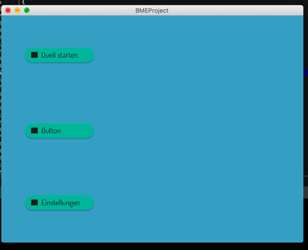
\includegraphics[width=5cm]{../img/screenshot_titlescreen.PNG} }}
\qquad
 \subfloat[Screenshot: Titlescreen 2]{{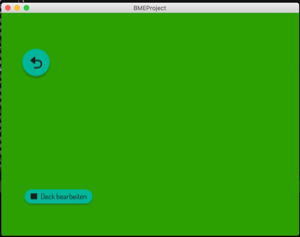
\includegraphics[width=5cm]{../img/screenshot_titlescreen_2.PNG} }}
\caption{Screenshots Titlescreen}%
 \label{fig:Screenshots Titlescreen}%
\end{figure}

In der render() Methode wird festgelegt, welcher Screen nach einem Klick auf den imageButtonBack angezeigt wird. In diesem Fall, soll das Startbildschirm erneut angezeigt werden. Nachdem mit einer If-Anweisung überprüft wird, ob der zurück Button geklickt wurde, wird das Startbildschirm angezeigt.  

Schließlich wurde durch diese Implementierung ermöglicht, die Spielumgebungen durch Klicks auf die Buttons anzusteuern und zwischen den Screens zu wechseln. 

\subsubsection{Imagebuttons für BattleScreen}
Anfangs wurden die Screens mit einer Hintergrundfarbe festgelegt. 
Allerdings war das nur vorübergehend. In diesem Semester erstellte Robert Sabo alles, was für den BattleScreen benötigt wurden.
Alle Bilder, die hierfür auf diesem Screen benötigen werden, wurden zunächst einmal in den Assets- beziehungsweise Visuals-Ordner eingefügt. Das Spielfeld sah anfangs an den Seiten leer aus. Das liegt daran, das alle Buttons hinzugefügt und richtig positioniert werden mussten. Das Endergebnis ist in Abbildung \ref{fig:Screenshot: BattleScreen mit ImageButtons} zu sehen.
\begin{figure}
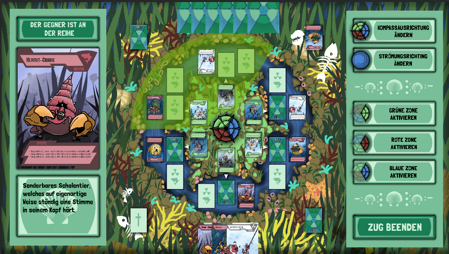
\includegraphics[width=0.5\textwidth]{../img/screenshot_battlescreen_buttons.PNG}
\caption{Screenshot: BattleScreen mit ImageButtons}
\label{fig:Screenshot: BattleScreen mit ImageButtons}
\end{figure}
Um testen zu können, ob der Klick auf den Button funktioniert, wurde zunächst einmal in der Console die Information „Zone successfully clicked“ wie folgt ausgegeben. \\
\begin{lstlisting}
450.0breite: 800.0
BATTLE SCREEN SHOWN
Zone successfully clicked
\end{lstlisting}

\subsubsection{Überarbeitung des Menüs im BattleScreen}
Um den Spieler das Spielen etwas zu erleichtern, wurden ein paar Hilfestellungen implementiert. Zunächst sollte der Spieler wissen, wer gerade an der Reihe ist. Hierfür wurde für die Klasse “Party” dem  „Spieler 1“ der Imagepath zu dem Asset „du\_bist.png“ zugeordnet. Dem „Spieler 2“ wurde der Imagepath zu dem Asset „gegner\_ist.png“ zugeordnet. Der Path wird der Klasse “BattleControl” übergeben. Dort wird die Methode showActivePlayer implementiert. Diese Methode zeichnet das Bild an der gewünschten Stelle. Die Methode wird in der Methode „changeActivePlayer“ ausgeführt.
Des Weiteren sollte der Spieler wissen, welche Effekte die unterschiedlichen Buttons im Spiel haben. Dafür wurde die Methode „setUserMessage“ in der Klasse „DetailView“ implementiert. Dieser Funktion wird jedes mal der String „userMessage“ übergeben, wenn der Spieler über einen Button, das Grab oder seine Handkarten fährt.
Folgende Objekte benötigten folgende User Message:
\begin{itemize}
\item Strömungsrichtung ändern Button - Die Strömung im Rücken ist vom Vorteil. Sie lässt dich zuerst Angreifen
\item Handkarten - Setze deine Einheit auf die gewünschte Kampfposition
\item Kompassausrichtung ändern - Drehe den Kompass um die Sektoren mit Strahlung auszusetzen. Die verschiedenen Strahlungen beeinflussen die Einheiten auf unterschiedliche Weise
\item Grab - Diese Einheiten stehen dir für den Kampf nicht mehr zur Verfügung
\item Rote  \& Blaue Strahlung Aktivieren Button - Deine Kreaturen und Phänomene werden durch die rote/blaue Strahlung zu wahren Kriegsmaschinen
\item Grüne Strahlung Aktivieren Button - Die Grüne Strahlung schafft dir mehr Raum um neue Einheiten in den Kampf zu senden
\item Zug beenden Button - Beende deinen Zug
\end{itemize}

Die Nachricht an den Spieler muss an der gewünschten Position, im gewünschten Absatzformat und mit automatischen Umbrüchen bei langen Texten angezeigt werden. Dies kann mit den Funktionen .setPosition, setWidth, .setHeight, .setAlignment und .setWrap aus dem Framework libGDX erfolgen. 
Um eine eigene Schriftart einzubinden wird der FreeTypeFontGenerator von libGDX benötigt. Dieser wandelt eine True Type Font in eine BitMap Font in der gewünschten Größe um. Für den Font muss ein linearer Filter für die Kantenglättung aktiviert werden.

Siehe im Git-Repository in den Commits:
\begin{itemize}
\item 11e47f46e37f4ab279a322218272dbd34607bd0b
\item 02d6bfa7794a80f599a048de649a22a8b060f047
\item db2c258eb297e9354fe680d54f02bee5e6bd0800
\end{itemize}

\subsubsection{Kartenauswahl}
Für die Auswahl einer bestimmten BattleCard und die damit verbundene Aktivierung bzw. Aktionsauslösung mussten erst entsprechende Vorbereitungen getroffen werden.
Zum einen benötigte die Klasse an sich einen InputListener des Typs “touchDown”, welcher für die Auswahl der Karte durch Anklicken benötigt wird. Das Hinzufügen des InputListeners stellte die Klasse Actor, von der die BattleCard erbt, über die Methode addListener bereit. Ihr musste nur die Klasse InputListener übergeben werden, bei der man direkt interne Anpassungen durchführen konnte. So wurde die von ihr beinhaltende Methode touchDown für unser Vorhaben genutzt, indem sie die von dem Klick betroffene Karte als “zuletzt angeklickte Karte” sicherte. Für eine flexiblere Verwendung der dadurch aktivierten Karte, wurde sie im BattleController als solche gesetzt und war damit dank Getter-Methoden auch von den restlichen Klassen abrufbar.

\subsubsection{Karte aus der Hand spielen}
Bei jedem Kartenspiel ist es wichtig, die Karte, welche aus der Hand gespielt wird, abzulegen. Um diese Funktionalität an der richtigen Stelle einbauen zu können, wurde zunächst einmal der Code analysiert. Mit Hilfe der Ausgabe auf der Consolen-Ausgabe, konnte ermittelt werden, welche Klassen und Methoden hierfür benötigt wurden. 

Die giveLastClickedBattledCard() Methode in der BattleControler Klasse gibt die lastClickedBattleCard, mit dem Rückgabetyp BattleCard, zurück. Mit Hilfe dessen, wurde zu aller erst ermittelt, ob die selecteCard null ist. Denn nur wenn eine Karte erst ausgewählt wird, kann diese auch wieder abgelegt werden. Nach einer weiteren if-Anweisung konnte mit Hilfe der Methoden addCard() und resetLastClicketBattleCard() die Funktionalität, die Karte aus der Hand zu legen, implementiert werden. Die folgenden Zeilen ermöglichen diesen Spielzug. 

\begin{lstlisting}
@Override public boolean touchDown(InputEvent event, float x, float y, int pointer, int button)
{
    BattleController battleController = FIELDABLE.giveBattleController();
    BattleCard  selectedCard     = battleController.giveLastClickedBattleCard();

    if (selectedCard != null) {
        addCard(selectedCard);
        battleController.resetLastClickedBattleCard();
    }
    return true;
}
\end{lstlisting}

Damit wurde somit dem Anwender die Option gegeben, seine Karte auf dem Spielfeld abzulegen. 

\subsubsection{TitleScreen ausbauen: zum BattleScreen navigieren}
Sobald das Projekt gestartet wurde, wurde uns der BattleScreen angezeigt. Daher musste der TitelScreen ausgebaut werden. Am Anfang des Semesters wurde diese Funktionalität zwar bereits programmiert, allerdings gab es während dem Semester Code-Änderungen. Das Resultat dieser Änderungen ergab, dass trotz eines Klicks auf den Button, der Anwender weiterhin den Titelbildschirm sah und somit nicht navigiert wurde. 

Dabei wurde festgestellt, dass der Verweis auf den BattleScreen nicht sofort funktionierte, weshalb der vorhandene Code analysiert wurde. Der TitelScreen erbt von AbstractScreen. Dieser enthält die Methode createController mit dem Parameter SpriteBatch spriteBatch. Allerdings muss diese Methode in der TitelScreen Klasse erweitert werden. Daher musste der Konstruktor der TitelController Klasse mit einem zweiten Parameter, dem TitelScreen titelScreen, ergänzt werden. Des Weiteren wurde im TitelScreen der return Wert von der creatController Methode angepasst. Schließlich funktionierte wieder der Verweis auf den BattleScreen. 

\subsubsection{Deckeditor}
Um dem Spieler die Möglichkeit zu verschaffen ein eigenes, individuelles Spielkartendeck zu erstellen, war anfangs ein Deckeditor geplant, der vom Titelscreen aus aufgerufen werden sollte. Die Klassen Deck, DeckScreen und DeckController wurden hierfür implementiert. Sie waren anfangs auch für interne Tests hilfreich, da sie alle Spielkarten hielten und dadurch der Zugriff auf Daten wie Kartenname oder Typ möglich war. Da die Priorität am Ende jedoch auf einer funktionierenden, visuell ansprechenden Spielfunktion lag, wurde der Deckeditor, und damit auch die Ausarbeitung der Deck-Klassen, auf Eis gelegt.

\subsubsection{Karten ziehen (Debug)}
Zur Visualisierung der Kartenziehung wurde vorerst vom Kartenstapel jeweils eine Karte auf das HandField verschoben.
Dafür musste die drawTopCard-Methode der Player-Klasse innerhalb des BattleControllers aufgerufen werden.
Dieser Aufruf musste nur noch mittels eines Impuls ausgelöst werden, für diesen Fall bot sich die von LibGDX bereitgestellte Tastendruckabfrage an:
\begin{lstlisting}
if (Gdx.input.isKeyJustPressed(Input.Keys.SPACE)) {
	activePlayer.drawTopCard();
}
\end{lstlisting}
Vorerst wurde diese Aktion mittels der Leertaste ausgeführt, wobei der Auslöser im Laufenden noch ausgearbeitet wurde.

\subsubsection{Visuelles Feedback innerhalb Eintrittsfelder}
Um dem Nutzer das Spielprinzip während seines Spielzuges zu erleichtern, bot sich eine visuelle Rückmeldung für die zum Ablegen von BattleCards ansteuerbaren Felder an. Um die Aufmerksamkeit des Nutzers also auf die möglichen Ablageorte zu lenken, wurde als Form der Kennzeichnung ein Asset in Form eines gelben Rahmens mit glühendem Effekt angefertigt. Dieses wird schließlich um das Feld oder die Felder pulsartig aufleuchten.
Der erste Schritt in der Implementierung dieser Funktion lag im Hinzufügen des Assets in alle Ablagefelder (EntryFields), wobei seine Transparenz auf Null gesetzt wurde. Optisch änderte sich am Spielfeld also noch nichts.
Bei diesem Schritt kam es jedoch zum Problem, dass sich das Verhalten des Ablagefeldes funktional veränderte, so wurde ein Mausklick auf dieses nicht mehr erkannt. Ein Kartenablegen auf dieses Feld war damit unmöglich.
Der Fehler lag hierbei in der Positionierung des Assets, das fälschlicherweise über den Feld-Actor gelegt wurde, der den Mausklick erhält. Dafür musste man die Assets auf eine niedrigere Ebene als die des Actors legen. Für diese Positionierung setzte man die Z-Position der Assets neu:
\begin{lstlisting}
int zCor = getZIndex() - 1;
glowBorder.setZIndex(zCor);
\end{lstlisting}

Der zweite Schritt wird durch den Mausklick auf die BattleCard angestoßen. Hier wird vorerst durch alle sechs Sektoren durchiteriert:

\begin{lstlisting}
public void activateSectorOfPlayer(Party party){
  for (Sector s : BATTLEFIELD.giveSectors()) {
     if (s.giveCommander().PARTY == party) {
        s.giveEntryField().showBorder();
     } else {
        s.giveEntryField().hideBorder();
     }
  }
}
\end{lstlisting}

Liegt dabei ein Sektor im Besitz des aktiven Spielers, so startet die vorgesehene Animation auf dem im Sektor enthaltenen Ablagefeld.
Für Animationen stellt LibGDX eigene Aktionen bereit. Für den gewünschten, pulsierenden Effekt wurde die “RepeatAction” gewählt, der man eine Ausblende- und Einblendefunktion übergeben muss:

\begin{lstlisting}
repeatAction.setAction(Actions.sequence(Actions.fadeOut(duration);
Actions.fadeIn(duration)));
\end{lstlisting}

Bei jedem Aufruf dieser Aktion werden diese beiden Funktionen einer Art Aktionsschleife hinzugefügt. Je länger diese Schleife wuchs, desto geringer wurde der prozentuale Anteil der Animationsdauer (Duration), daher verschnellerte sich bei jedem Klick die Rahmenanimation des Ein- und Ausblendens. Aus diesem Grund musste diese Aktionsschleife vor jedem Aufruf zuerst geleert werden:

\begin{lstlisting}
glowBorder.getActions().clear();
\end{lstlisting}

Diese Methode wird auch für das Beenden der Animation verwendet. Dieser Fall tritt immer dann ein wenn der Spieler aktuell keine BattleCard aktiviert hat, also wenn er entweder eine Karte abgelegt oder sie durch Klicken auf das Spielfeld unselektiert hat.
Das Beenden der Animation lässt den Rahmen jedoch nicht verschwinden, sondern fügt ihn in seiner aktuellen Transparenz, die zwischen Eins (fadeIn) und Null (fadeOut) variiert, der Stage hinzu. Für das endgültige Beenden der visuellen Rückmeldung muss die Transparenz der Assets wieder auf Null gesetzt werden:

\begin{lstlisting}
glowBorder.setColor(1,1,1,0);
\end{lstlisting}

\subsubsection{Klickanimation der Buttons}
Für die visuelle Bestätigung der Durchführung eines Klicks wurden die Spielefeldbuttons um ein Asset erweitert. Der Aufruf des ImageButton-Konstruktors mit zwei Parametern, imageUp und imageDown, ermöglicht es die Buttongrafiken während eines Mausklicks, als auch nach dieser Aktion, zu setzen. Das neu hinzugefügte Asset beinhaltet die Buttongrafik in einer schwächeren Belichtung:

\begin{lstlisting}
final Texture     BUTTON_RED_DOWN = new Texture("core/assets/visuals/buttons/3_rotbuttonSmall_down.png");
final ImageButton RED_BUTTON = new ImageButton(new TextureRegionDrawable(new TextureRegion(BUTTON_RED)), new TextureRegionDrawable(new TextureRegion(BUTTON_RED_DOWN)));
\end{lstlisting}

\subsubsection{Deselektion der BattleCard}
Selektiert der Player eine Handkarte und entscheidet sich daraufhin um, weil er lieber eine oder mehrere andere Aktionen durchführen möchte, wird der Buffer der letzten geklickten Karte geleert und ihre Aktivierung damit aufgehoben. Generell geschieht dies bei jedem Mausklick außerhalb einer BattleCard.
Benötigt wird hier also eine Abfrage, ob sich auf geklickter Position ein Actor befindet, der wiederum von einer BattleCard gehalten wird.
Mit der hit-Methode der Stage-Klasse können wir dies leicht überprüfen. Diese benötigt lediglich die Koordinaten des Mausklicks, um einen dort positionierten Actor auszugeben. Dieser wird anschließend auf seine Zugehörigkeit geprüft, die nicht der BattleCard angehören darf:

\begin{lstlisting}
if (Gdx.input.justTouched()) {
	Stage stage = giveStage();
	Vector2 vector = new Vector2(Gdx.input.getX(), Gdx.input.getY());
	stage.screenToStageCoordinates(vector);
	Actor clickedActor = stage.hit(vector.x, vector.y, true);
	if (clickedActor != null){
		if(!(clickedActor instanceof BattleCard)) {
			resetLastClickedBattleCard();
		}
	}
}
\end{lstlisting}

\subsubsection{Spielfeld}
Um das Spielgeschehen überhaupt zu gestalten, bedarf es eines Spielfeldes, auf dem sich alle Spielzüge abspielen können.
Dies darf man gerne mit einer Art „Schlachtfeld“ in einem kriegerischen Strategiespiel vergleichen, auf dem es einzunehmende Basen, die sogenannten „Quartiere“ gibt. Ziel einer Partie ist es, sämtliche Basen des Gegenspielers für sich zu gewinnen, indem alle verteidigenden Kreaturen besiegt und somit vom Feld genommen werden.
Zum Spielfeld von EDWARDS BIOTOPE gehören Sektoren, Zonen und die darin geschehende Feldpositionierung. Die dafür benötigten Programmelemente wurden von Robert, Pamela, Gabriel, Cigdem, Manuela und Felix implementiert.

\textbf{Sektoren}
Das Spielfeld von EDWARDS BIOTOPE ist in sechs Sektoren aufgeteilt, die jeweils ein Quartier und drei Kreaturen und Phänomene halten können. Die im Spiel gelegten Karten werden wiederum den verschiedenen Feldern zugeordnet, die im jeweiligen Sektor angelegt sind.
\begin{lstlisting}
public Sector(Battlefield battlefield, Vector2 field1Vector, Vector2 field2Vector, Vector2 field3Vector,
      Vector2 quarterFieldVector)
{
   super();
   BATTLEFIELD = battlefield;
   FIELDS.add(new Field(this, quarterFieldVector));
   FIELDS.add(new LeadField(this, field1Vector));
   FIELDS.add(new EntryField(this, field2Vector));
   FIELDS.add(new EndField(this, field3Vector));
}
\end{lstlisting}

Es wird außerdem ausgegeben, welche Sektoren vor bzw. nach dem aktuellen Sektor stehen.

\begin{lstlisting}
public Sector givePreviousSector()
{
   return BATTLEFIELD.givePreviousSectorOf(this);
}

public Sector giveNextSector()
{
   return BATTLEFIELD.giveNextSectorOf(this);
}
\end{lstlisting}

Siehe im Git-Repository in den Commits:
\begin{itemize}
\item daf1fc139ee620220bbe36340e67b0e3bcbeada2
\item e68492971171565a17d499ab5675c5032eb09542
\item a936f5cfb03662dd957ca27a2ecf8b86e4da1c9a
\end{itemize}

\textbf{Zonen}
Es erstrecken sich drei verschiedenfarbige Zonen über das Spielfeld: Rot, Grün und Blau. Jede Zone enthält jeweils zwei Sektoren. Die Zone selbst ist als eine Aufzählung angelegt und kann je nach momentan liegender Farbe aktiviert werden.
\begin{lstlisting}
public enum Zone
{
   // ===================================
   // ENTRIES
   // ===================================

   RED,
   GREEN,
   BLUE;

   // ===================================
   // ATTRIBUTES
   // ===================================

   private boolean activated;

   // ===================================
   // CONSTRUCTORS
   // ===================================

   Zone()
   {
      activated = false;
   }

   // ===================================
   // ATTRIBUTES
   // ===================================

   public static Zone giveZoneByColorIndex(int index)
   {
      for (Zone zone : values()) {
         int ordinal = zone.ordinal() * 2;
         if (ordinal == index || (ordinal + 1) == index) {
            return zone;
         }
      }
      return null;
   }

   public boolean isActivated()
   {
      return activated;
   }

   public void activate()
   {
      activated = true;
   }

   public void deactivate()
   {
      activated = false;
   }
}
\end{lstlisting}

Siehe im Git-Repository in den Commits:
\begin{itemize}
\item cfb3bf3736c1e90fc7144eb4a110ab580337df68
\item 9b915960bfaf07586067aaa2ac92173d0700350d
\item 16261f7ae75d97aedf791c6af081314f70f0ebdd
\item c83d620c1d9bd22af5b58b22c683b0d596c66783
\end{itemize}

\textbf{Feldpositionierung}
Für das Spielgeschehen spielt die Feldpositionierung eine entscheidende Rolle. Hiermit wird angegeben, auf welchem Feld sich eine Karte befindet, oder ob ein Feld leer ist. So hat ein Sektor ein Feld für das Quartier und drei Felder auf denen Kreaturen abgelegt werden können, wovon das erste das Eintrittsfeld darstellt. Über dieses Feld werden die Kreaturen in das Spielgeschehen geschickt. Sollte die grüne Zone aktiviert werden, kann die Kreatur dann auf eines der anderen Felder weitergeschoben werden, damit das Eintrittsfeld wieder frei wird für neu hinzukommende Karten.

\begin{lstlisting}
@Override public Field giveCurrentFieldOfBattleCard(BattleCard battleCard)
{
   for (Field field : FIELDS) {
      if (field.giveCards().contains(battleCard)) {
         return field;
      }
   }
   return null;
}
\end{lstlisting}

Mit der folgenden Funktion wird von den Sektoren abgefragt, ob das jeweilige Feld eine Karte hält oder nicht. Basierend auf diesen Flags, kann das Battlefield die Informationen dann dem Kontext entsprechend verarbeiten.

\begin{lstlisting}
public boolean hasBattleCard(BattleCard battleCardToHave)
{
   for (Field field : FIELDS) {
      if (field.giveCards().contains(battleCardToHave)) {
         return true;
      }
   }
   return false;
}
\end{lstlisting}

Des Weiteren wird ausgegeben, welches Feld mit welchen Karten belegt ist. Per get() findet hier eine eindeutige Zuweisung an der jeweiligen Stelle der zugrundeliegenden ArrayList ab. So können wir einen Trading-Card Spieltisch später mit fest zugewiesenen Slots für Karten verstehen und letztendlich grafisch übersichtlich präsentieren.

\begin{lstlisting}
public Field giveQuarterField()
{
   return FIELDS.get(0);
}

public ArrayList<RingField> giveRingFields()
{
   ArrayList<RingField> ringFields = new ArrayList<RingField>();
   ringFields.add(giveLeadField());
   ringFields.add(giveEntryField());
   ringFields.add(giveEndField());
   return ringFields;
}

public LeadField giveLeadField()
{
   return (LeadField)FIELDS.get(1);
}

public EntryField giveEntryField()
{
   return (EntryField)FIELDS.get(2);
}

public EndField giveEndField()
{
   return (EndField)FIELDS.get(3);
}
\end{lstlisting}

In welche Richtung die Karten auf dem Feld positioniert werden, wird an der aktuellen Strömungsrichtung ausgemacht. Sie dient durch ihre Sortierung der Array-Liste später auch dazu, Angriffsrichtungen im Stellungsspiel um die Quartierkarten zu bestimmen.
Man drückt im Interface am Anfang der Runde auf einen optionalen Schalter und dreht damit den Ablauf entweder im, oder gegen den Urzeigersinn. Das bestimmt dann, wer für eine Kreaturen-Karte das nächste mögliche Angriffsziel sein kann.

\begin{lstlisting}
private ArrayList<BattleCard> reverseCardOrder(ArrayList<BattleCard> list)
{
   Collections.reverse(list);
   return list;
}

public BattleCard giveQuarter()
{
   return FIELDS.get(0).giveCards().get(0);
}

public ArrayList<RingField> giveOrderedRingFields()
{
   ArrayList<RingField> orderedRingFields = giveRingFields();
   BATTLEFIELD.COMPASS.giveStream().orderRingFields(orderedRingFields);
   return orderedRingFields;
}
\end{lstlisting}

Siehe im Git-Repository in den Commits:
\begin{itemize}
\item daf1fc139ee620220bbe36340e67b0e3bcbeada2
\item e68492971171565a17d499ab5675c5032eb09542
\item a936f5cfb03662dd957ca27a2ecf8b86e4da1c9a
\end{itemize}

\subsubsection{Musik und Soundeffekte}
LibGDX bietet eine Musikschnittstelle, mit der man Musik und Soundeffekte leicht in das Spiel einbinden kann. Dafür gibt es die zwei Klassen “Music” und “Sound”. Bei einer Audiodatei, deren Länge ein paar Sekunden übertrifft, handelt es sich um eine Music-Klasse.  Es ist zu bevorzugen, die Datei von der Festplatte zu streamen, anstatt sie vollständig in den Arbeitsspeicher zu laden. Die Sound-Klasse bedient Soundeffekte, wie kleine Audio-Samples, die in der Regel nicht länger als einige Sekunden dauern und bei bestimmten Spielereignissen wiedergegeben werden sollen, wie zum Beispiel beim Drücken eines Buttons, beim Kartenziehen oder beim Drehen des Kompasses. Soundeffekte können in verschiedenen Formaten gespeichert werden. LibGDX unterstützt MP3-, OGG- und WAV-Dateien. Die benötigten Audio-Dateien liegen dabei im Assets-Ordner.
Um die Musik in das Spiel zu laden, muss eine Instanz der Music-Klasse generiert werden. Dies passiert in der BMEProjekt-Klasse, damit man die Musik und Soundeffekte in allen Klassen benutzen kann:

\begin{lstlisting}
public static Music music = Gdx.audio.newMusic(Gdx.files.internal("core/assets/audio/music.mp3"));
\end{lstlisting}

Die Attribute der Music-Klasse erlauben die Anpassungen einiger Einstellungen, wie beispielsweise die Veränderung der Lautstärke und die Setzung der Audio-Datei auf Wiederholung:

\begin{lstlisting}
music.setVolume(1.0f);
music.setLooping(true);
\end{lstlisting}

Das Abspielen der Musikinstanz funktioniert wie folgt:

\begin{lstlisting}
music.play();
\end{lstlisting}

Um Ressourcen freizugeben wird die Musikinstanz in der BMEProjekt-Klasse entsorgt, sobald sie nicht mehr benötigt wird:

\begin{lstlisting}
music.dispose();
\end{lstlisting}

Die Soundeffekte werden ähnlich implementiert und wie folgt abgespielt: 
\begin{lstlisting}
BMEProject.streamSound.play(0.2f);
\end{lstlisting}

Dadurch wird der Soundeffekt einmal mit der Lautstärke von 20 \% wiedergegeben. Die Methode .play(); wird beim Eintreten bestimmter Ereignissen gesetzt.

\subsubsection{XML befüllen}
Um der Klasse Cards ihre Werte zuzuweisen, wird ein XML benötigt mit allen relevanten Informationen. Jede Karte benötigt eine ID, cardName, cardType, cardEffect, cardDescription und den cardIllustrationFilePath. Diese Informationen wurden für 44 Karten hinterlegt.
Siehe hierzu den Commit:
\begin{itemize}
\item 1f719baad08daf434cbb0c69186e068338359ade
\end{itemize}

\subsubsection{Effekte}
Da jede Karte mehrer Effekte bekommen sollte, wurde eine XML mit 10 Effekten erstellt.
Der bisherige XML-Reader liest bisher die CARDS XML aus und musste deshalb erweitert werden, um die Effekte XML auszulesen. Jeder Effekt hat einen Integer Wert, mit der eigener ID.  Zusätzlich einen String, der den Effekt in einem Satz beschreibt.
Um die Effekte den einzelnen Karten zu zuzuordnen, wurden die Karten im XML um den Tag <Effects> erweitert. In diesem Tag können die IDs der Effekte als Integer Wert eingetragen werden. Die Effekte werden mit der Karte verbunden, indem die Klassen „Card“ und „DeckCard“ um den Typ Effekt erweitert werden. Damit die Effekte angezeigt werden, wurde eine Methode implementiert, die die Karten in größerer Auflösung anzeigt. Beim Drüberfahren mit der Maus werden die Effekte, Typ und Beschreibung als Text anzeigt.
Die Effekte wurden jedoch gestrichen, da die Konzeption der einzelnen Effekte nicht abgeschlossen war. Außerdem konnte die Implementierung zeitlich nicht bewältigt werden. Der Branch wurde deshalb im Git-Repository nicht dem Master Branch hinzugefügt.
Siehe im Git-Repository den Branch: 70 76 KartenDetailsAnzeigen KartenAssets

\subsubsection{Siegesbedingung}
Um den Spieler zu signalisieren, wer der Gewinner ist, fehlte noch eine Methode mit einer Benachrichtigung über den Sieg. Nachdem ein Quartier den Besitzer gewechselt hat, wird über die sechs Quartiere auf dem Spielbrett iteriert. In der Iteration wird geprüft, welchem Spieler die Quartiere gehören. Besitzt ein Spieler alle sechs Quartiere, hat dieser gewonnen. Nach dem Erfüllen der Bedingung wird ein Bild angezeigt mit der Nachricht „du hast gewonnen“ oder „du hast verloren“. Zusätzlich werden Buttons eingefügt,  um ein neues Spiel zu starten und um zurück in das Hauptmenü zu gelangen. 
Siehe im Git-Repository in den Commits:
\begin{itemize}
\item c390e51a6058673c1509ec47513f5e58ba560900
\item 649f98e2344ba5429391f988e76dc903e2d58e08
\item 7bcdccc49363fca3ac3529966aa51384e178c47c
\item f634203a5dd291874886739790f981ed42f5fdc8
\end{itemize}

Die entsprechende Logik wurde von Pia Korndörfer zuerst in den Klassen Battleflied und BattleController umgesetzt. Da es sich hierbei fachlich um einen eigenen Screen handelt musste der Code hierfür in einen neuen Screen umgezogen werden. Hierfür implementierte Sebastian Beck einen entsprechenden EndOfGameScreen und einen passenden Controller und übernahm die grundsätzliche logik. Die Besonderheit bei diesem Screen ist jedoch im vergleich zu den anderen, dass dieser nicht initial mit den anderen Screens im Projekt gebaut werden kann, da er vom Spielergebnis abhängig ist. Jedoch werden gleichzeitig die einzelnen Screens und Aufrufe über die zentrale Klasse "BMEProject" gesteuert. Hierzu wurde die BMEProject-Klasse um die Methode "setEndOfGameScreen()" erweitert. Diese erwartet ein vorbereitetes Objekt der "EndOfGameScreen"-Klasse, welches bereits mit einem Booealn "isWin" beladen ist um einen Gewinn oder Verlust anzuzeigen. \\
\textbf{BattleController:}
\begin{lstlisting}
if (allyCounter == 6) {
	endOfGameScreen = new EndOfGameScreen(BME_PROJECT, this, true);
	BME_PROJECT.setEndOfGameScreen(endOfGameScreen);
	return true;
}
\end{lstlisting}
\textbf{BMEProject:}
\begin{lstlisting}
public void setEndOfGameScreen(EndOfGameScreen endOfGameScreen)
{
	setScreen(endOfGameScreen);
}
\end{lstlisting}

\subsubsection{Starter Deck mit drei Quartieren}
Jeder Spieler darf in dem eigenen Deck Maximal drei Quartiere haben. Bisher wird das Kartendeck zufällig mit einem Random Number Generator generiert ohne dabei eine Obergrenze für Quartiere zu berücksichtigen. Die Quartiere in Cards\_XML haben die ID 1 bis 5 und die restlichen Kartentypen von 6 bis 44. Deshalb wurde der Random Number Generator aufgeteilt. Zunächst werden zufällig drei Zahlen von 1 bis 5 gezogen, anschließend werden 37 Zahlen zwischen 6 bis 44 gezogen. Die Kombination der Karten IDS wird beim Spielstart als Deck für den Nutzer gespeichert.
Siehe im Git-Repository in dem Commit:
\begin{itemize}
\item c390e51a6058673c1509ec47513f5e58ba560900
\end{itemize}

\subsubsection{Auflösung auf des Title Screens und des BattleScreens auf HD anpassen}
Bisher ist das Spielfeld auf eine Auflösung 800x450 Pixel konfiguriert. Diese Einstellung wurde auf Full HD Auflösung 1920x080 angepasst. Alle Regionen für die Karten waren absolut positioniert. Deshalb mussten alle Regionen neu positioniert und skaliert werden, um die volle Auflösung zu nutzen. 
Die Assets waren nicht auf die HD-Auflösung angepasst und werden entweder vergrößert oder verkleinert angezeigt, dadurch entsteht ein Qualitätsverlust. Da EDWARDS BIOTOPE Full HD unterstützen soll, wurden die Assets auf die tatsächliche Größe angepasst. Um die tatsächlichen Größen auszulesen, wurde ein Screenshot des aktuellen Spiels in Adobe Photoshop vermessen und die benötigten Größen aufgeschrieben. Anschließend wurden die Assets in der tatsächlichen Größe erneut gespeichert und in das Spiel eingebunden. Die Spielkarten werden in zwei Größen benötigt. Einmal als kleine Version für das Spielbrett und eine große Version für die Detail-Ansicht. Deshalb muss die Klasse “Cards” um zwei Strings erweitert werden. Zum einen den LLUSTRATION\_FILE\_PATH dieser Path setzt sich "core/assets/visuals/cards/large/" und der Variable illustrationFilePath zusammen. Zusätzlich der ILLUSTRATION\_FILE\_PATH\_SMALL, dieser setzt sich aus "core/assets/visuals/cards/small/" und der Variable illustrationFilePath zusammen. Die Variable illustrationFilePath weist der XML Reader aus dem Card XML zu. Die Klasse “Battle Card” verwendet als Texturen für die Spielkarten den Pfad den ILLUSTRATION\_FILE\_PATH\_SMALL und die DetailView ILLUSTRATION\_FILE\_PATH. 
Die Anzeige war nach den Anpassungen noch nicht zufriedenstellend, da LibGDX Texturen ohne Kantenglättung anzeigt.
Siehe hierzu die Commits:
\begin{itemize}
\item 8ccd2046db2a7def1d17a7988afe598631f64f7b
\item a0bab3abbb009b004659399adbbc854ee6932e8e
\item 1dea80495d1dc5ba55e9909326146ac56540672d
\item 90859da52af88b69d243b6d072f287102e0ca21e
\item dde09c88d28081d813a9c581a4425b7425eb8a98
\item 14ca0dd54308280139d0dac3d7e6e86d334a803f
\end{itemize}

\subsubsection{Anti Aliasing hinzufügen}
LibGDX bietet die Funktion .setFilter für Texturen an. Hierfür muss der Filter von „Nearest“ auf „Linear“ angepasst werden, um die Kanten der Assets zu Glätten. Deshalb wurde der Code nach allen Texturen durchsucht und für jede Textur die Funktion
\begin{lstlisting}
TEXTUR.setFilter(Texture.TextureFilter.Linear,Texture.TextureFilter.Linear);
\end{lstlisting}
hinzugefügt.
Siehe hierzu den Commit:
\begin{itemize}
\item 86617498da70acabe885862ce9db573342b08d6e
\end{itemize}

\subsubsection{Camera Handle für Variable Bildschirmgrößen}
LibGDX hat schon eine vorgefertigte Camera-Klasse, die man benutzen kann. Es gibt 2 Subklassen und zwar die OrthographicCamera und PerspectiveCamera. Bei der Orthographic Camera gibt es keine Perspektive, sondern alle Längen bleiben gleich egal von welchem Winkel man sie betrachtet.
Für unser Spiel ist eine Orthographic Camera am sinnvollsten, weil wir keine Tiefen mit 3D-Meshes im Spielfeld haben.
Die Implementierung der Kamera übernimmt die Renderer-Klasse
\begin{lstlisting}
private final SpriteBatch SPRITE_BATCH;
private Viewport viewport;
private Camera camera;
private Stage stage;
Renderer(SpriteBatch spriteBatch)
{
   SPRITE_BATCH = spriteBatch;
   camera = new OrthographicCamera();
   viewport = new FitViewport(1920f, 1080f, camera);
   camera.position.set(1920 / 2f, 1080 / 2f, 0f);
}
\end{lstlisting}
Als Viewport wird ein FitViewPort gewählt mit Full-HD Auflösung. Es gibt in LibGDX verschiedene Viewports z.B. StretchViewport, FillViewport, ScreenViewport usw. , der FitViewport
macht keine Verzerrung, d.h. Egal in welche Größe ich das Fenster skaliere, wird das Spiel nie verzerrt. Schwarze Ränder füllen die Ränder auf, falls das Format des Fensters nicht mit dem Format des Spiels zusammenpasst. Die Position der Kamera ist die Mitte des Bildschirms, also 1920/2 für X und 1080/2 für Y. In Edwards Biotope braucht es nur eine statische Kamera die auf einer Position bleibt. Im Gegensatz zu Zelda, wo sich die Kamera mit dem Spieler bewegt.
Die Render-Klasse hat ihre eigene Render-Methode. Die Methode bekommt bei jedem Render-Durchgang die stageToRender zugewiesen, das ist die Stage BattleScreen oder Titlescreen zum Beispiel, und der Viewport wird gesetzt. Das passiert 60 mal in der Sekunde.
\begin{lstlisting}
void render(Stage stageToRender)
{
   stage = stageToRender;
   stage.setViewport(viewport);
   Gdx.gl.glClearColor(0f, 0f, 0f, 0f);
   Gdx.gl.glClear(GL20.GL_COLOR_BUFFER_BIT);
   stage.draw();
}
\end{lstlisting}

\subsubsection{Server Kommunikation Testing mit Router und Lokal}
Die Implementierung, dass 2 Spieler am gleichen PC mit 2 Fenstern spielen können wurde bereits in einem frühen Stadium vom Spiel umgesetzt und kann als über die Projektzeit weiter führende Aufgabe in dem jetzigen Stand des Spiels, bei dem beide Spieler am gleichen Computer und im gleichen Fenster spielen, integriert werden. Dazu benötigt es nur der richtigen Events, die geschrieben werden müssen, um die Server-Kommunikation zu ermöglichen.
Das Testing mit einem Handelsüblichen Router ist ähnlich dem Testing an einem Computer, man muss nur einige Parameter in der Software umstellen.
Sowie beim Multiplayer auf einem System verwenden wir IO-Sockets mit einem Node-JS-Server.

Die nötige Installationen sind folgend beschrieben:
\begin{itemize}
\item NodeJS.org öffnen
\item z.B v10.14.2 LTS Downloaden
\item NodeJS installieren
\item Auf Mac: Terminal öffnen und „node —version“ eingeben. Wenn v10.14.2 als Antwort kommt
war die Installation erfolgreich, falls nicht ist es höchstwahrscheinlich, dass der Computer den
Pfad zu NodeJS nicht kennt
\item Server starten: Im Terminal „node index.js“ eingeben. Hierfür muss man zum Verzeichnis
wechseln wo index.js abgespeichert ist. Im Projektverzeichnis liegt dieses unter: bmeproject/game/bmeProject/MultiplayerDemo/Server
Note: index.js ist eine selbsterstellte Javaskript-Datei in die den Server definiert(dessen Events usw.)
\end{itemize}
Um Lauffähigkeit herzustellen muss ggf. lokal noch Socket.io installiert werden. Eine ausführliche Anleitung hierfür befindet sich im Anhang. 

Da es zum Testing keinen extra Server gab, wird ein PC, der das Spiel ausführt, zum Server gemacht. Das nennt sich Hosting und wird in Online-Spielen oft verwendet. Ein PC hat in seiner connectSocket die Localhost-Adresse eingetragen von sich selbst. Der andere PC hat die IP dieses PCs im Lokalen Netzwerk in seiner connectSocket()-Methode eingetragen. Diese IP ist beispielsweise 192.168.0.7. Beide Computer werden vorher mit dem Router verbunden per LAN-Kabel für optimale Geschwindigkeit.

\subsubsection{Zerstören von Karten}
Die Karten, die auf dem Spielfeld vom Gegner besiegt werden, müssen auf dem Friedhof landen, wenn es sich um Kreaturen oder Phänomene handelt. Quartiere werden nicht auf dem Friedhof abgelegt, sondern eingenommen vom Gegner. Die Kreaturen-Klasse und die Phänomenen-Klasse haben die gleiche getDestroyed()-Methode implementiert.

\begin{lstlisting}
@Override public void getDestroyed()
{
   BMEProject.destroySound1.play(0.5f);
   Field graveyard = PLAYER.giveGraveyard();
   graveyard.addBattleCard(this);
}
\end{lstlisting}

In dieser Methode wird dem Graveyard die BattleCard hinzugefügt mit dem Aufruf von addBattleCard(this). Außerdem wird für die Spielästhetik ein Sound abgespielt.
Da jeder Spieler seinen eigenen Friedhof hat, muss dieser erst abgefragt werden mit PLAYER.giveGraveyard(). Im Spiel ist der Graveyard ein Field, das einem Spieler zugeweisen ist. Die giveGraveyard()-Methode von Player gibt das Field aus einer Liste zurück, das für den Friedhof dieses Spielers steht. Alle Fields vom Spielfeld sind in einer Liste vorhanden und jedes Feld kann addressiert werden.

\begin{lstlisting}
public Field giveGraveyard()
{
   return FIELDS.get(2);
}
\end{lstlisting}

Zu der Methode addBattleCard() ist die Beschreibung etwas umfangreicher. Es hört sich einfach an was die Methode macht, dennoch muss man einige Abfragen machen.
Man hat ein currentField und einen FIELD\_USER. Man muss durch die Klassenhierarchie durchgehen. Man fragt den FIELD\_USER auf welchem Feld die mitgebene BattleCard sich befindet. Es kann auch sein, dass die BattleCard sich noch auf keinem Feld befindet. In den meisten Fällen ist das jedoch nicht so. Wenn das currentField also nicht null ist, wird die BattleCard von ihrem jetzigen Field entfernt mit removeCard(battleCardToAdd). Neben dieser Prüfung ist es auch wichtig nach der Existenz der Karte zu schauen. Wenn die Karte existiert wird sie der Liste CARDS hinzugefügt.

\begin{lstlisting}
public void addBattleCard(BattleCard battleCardToAdd)
{
   Field currentField = FIELD_USER.giveBattleController().giveCurrentFieldOfBattleCard(battleCardToAdd);
   if (currentField != null) {
      currentField.removeCard(battleCardToAdd);
   }
   if (battleCardToAdd != null) {
      CARDS.add(battleCardToAdd);
   }
   update();
}
\end{lstlisting}

Für die getDestroyed()-Methode des Quartiers müssen andere Abfragen und Befehle ausgeführt werden, deswegen ist diese Methode anders als die Kreatur- und Phänomen-Methode. Am Rande sei erwähnt, dass der Sound auch ein anderer ist und in deutlich niedrigerer Lautstärke.
Quatiere haben einen Kommandeur(commander). Der commander ist der Spieler, der das Quartier gerade kontrolliert. In der Methode wird dem commander der Gegenspieler des derzeitigen commanders vom Quartier zugewiesen. In dieser Methode wird auch ein currentField angelegt.
Dies dient dazu das currentField zu updaten.

\begin{lstlisting}
@Override public void getDestroyed()
{
   BMEProject.destroySound2.play(0.1f);
   commander = PLAYER.BATTLE_CONTROLLER.giveOppositePlayerOf(commander);
   Field currentField = giveCurrentField();
   if (currentField != null) {
      currentField.update();
   }
   PLAYER.BATTLE_CONTROLLER.checkForWin();
}
\end{lstlisting}

\subsubsection{Handhabe aktive Spieler}
Der BattleController ist verantwortlich für den Spielablauf während eines Tuniers von 2 Spielern. Der BattleController muss wissen welcher Spieler am Zug ist, damit er die Methoden beim richtigen Spieler ausführt. Zum Beispiel wäre es schlecht, wenn der BattleController beim Beginn eines Zuges von einem Spieler für den Gegenspieler die Methode drawTopCard() ausruft anstatt des derzeitigen aktiven Spieler. Bei diesem Fall würde der BattleController dem gerade nicht am Zug befindlichen Spieler eine neue Karte auf die Hand geben. Dies würde einen flüssigen Spielablauf so gut wie unmöglich machen, deswegen braucht man eine Instanz für den aktiven Spieler.

\begin{lstlisting}
private Player activePlayer;
\end{lstlisting}

Bei unserem Spiel gibt es genau 2 Spieler. Beide Spieler haben eine Nummer und zwar Spieler 1 und Spieler 2. Am Anfang von einem Spiel soll Spieler 1 der aktive Spieler sein.

\begin{lstlisting}
PLAYER_1 = new Player(this, Party.ALLY);
PLAYER_2 = new Player(this, Party.ENEMY);
activePlayer = PLAYER_1;
activePlayer.beginTurn();
\end{lstlisting}

Wer Spieler 1 und wer Spieler 2 ist, ist durch die Aufteilung des Spielfeldes festgelegt. Der Spieler der seine Hand auf der unteren Hälfte des Bildschirmes hat, ist der Spieler 1. Spieler 2 ist dementsprechend der Spieler auf der oberen Hälfte.

\begin{figure}[h]
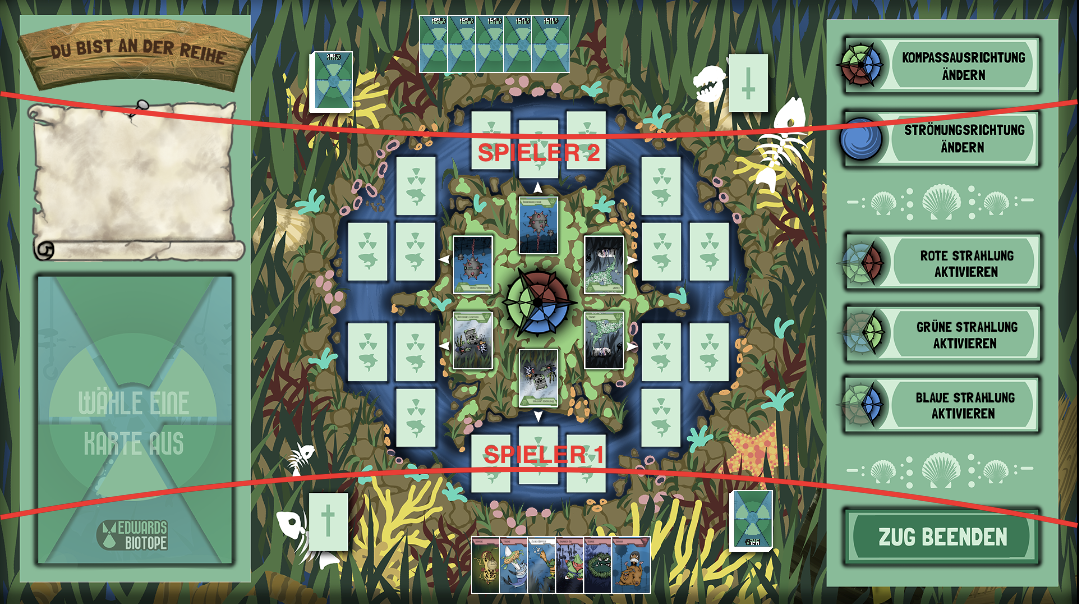
\includegraphics[width=1\textwidth]{../img/screenshot_spielfeldeinteilung.PNG}
\caption{Screenshot: Spielfeld mit Spielerbereichen}
\label{fig:Screenshot Spielfeld Spielerbereiche}
\end{figure}

Jetzt funktioniert es, dass die Methoden vom activePlayer, der Spieler 1 ist, aufgerufen wird. Wenn Spieler 1 seinen Zug beendet ist er dennoch activePlayer, aber dies ist ja nicht was wir wollen. Wir brauchen eine neue Methode die den aktiven Spieler von Spieler 1 zu Spieler 2 ändert und auch in anderer Richtung.

Diese Methode muss den activePlayer kennen und diesen neu zuweisen. ActivePlayer soll also Spieler 2 zugewiesen werden.

Den activePlayer kennt die Methode, weil activePlayer eine Instanz-Variable ist. Dennoch besteht das Problem, dass man nicht einfach Spieler 2 dem activePlayer zuweisen kann. So funktioniert die Methode nur in eine Richtung und nicht rückwärts. Es wird eine weitere Methode benötig, die den gerade nicht aktiven Spieler ausgibt, also den Gegenspieler. GiveOppositePlayerOf(Player player) wäre so eine Methode.

\begin{lstlisting}
public Player giveOppositePlayerOf(Player player)
{
   if (player == PLAYER_1) {
      return PLAYER_2;
   } else {
      return PLAYER_1;
   }
}
\end{lstlisting}

Die Abfrage ist recht trivial. Man gibt der Methode den activePlayer mit. Wenn der activePlayer Player 1 ist, wird der Player 2 zurückgegeben. Beim umgedrehten Fall wird Spieler 1 zurückgegeben. Nun können wir dahin zurück den activePlayer neu zuzuweisen. Die Methode changeActivePlayer() macht genau dies in Kombination mit getOppositePlayer(Player player).

\begin{lstlisting}
public void changeActivePlayer()
{
   resetLastClickedBattleCard();
   Zone.RED.deactivate();
   Zone.GREEN.deactivate();
   Zone.BLUE.deactivate();
   setTurnUnstarted();
   BUTTON_VIEW.fadeInZoneButtons();
   Player nextPlayer = giveOppositePlayerOf(activePlayer);
   nextPlayer.beginTurn();
   activePlayer = nextPlayer;
   updateAllFields();
   showActivePlayerMessage();
}
\end{lstlisting}

In der Methode wird eine neue Variable nextPlayer angelegt. Dieser wird der return-Wert von giveOppositePlayerOf(activePlayer) zugewiesen. Dem activePlayer wird dann nurnoch der nextPlayer-Wert zugewiesen und schon ist das Problem gelöst.
Neben dem Opposite Player kann man natürlich auch den activePlayer, falls er gebraucht wird, ausgeben lassen.

\begin{lstlisting}
public Player giveActivePlayer()
{
   return activePlayer;
}
\end{lstlisting}

Wenn ein Spieler am Zug ist, müssen auch seine eigenen Sektoren aktiviert werden und die vom Gegener deaktiviert, damit er nur auf seine eigenen Sektoren Karten legen kann. Dafür benötigt man auch den activePlayer und man geht bei ALLY von Spieler 1 aus und bei ENEMY von Spieler 2.

\begin{lstlisting}
public void activateSectorOfPlayer(Party party){
   for (Sector s : BATTLEFIELD.giveSectors()) {
      if (s.giveCommander().PARTY == party) {
         s.giveEntryField().showBorder();
      } else {
         s.giveEntryField().hideBorder();
      }
   }
}
\end{lstlisting}

\subsubsection{Felder}
Unser Spielfeld ist in 6 Sektoren aufgeteilt. Jeder Sektor hat 4 Fields auf denen jeweils eine Karte abgelegt werden kann. Das Field muss wissen ob eine Karte auf ihr liegt oder ob sie frei ist. Das Field an sich hat X- und Y-Koordinaten sowie eine Breite und eine Höhe. Eine Karte wird in einem sogenannten Pile innerhalb des Fields abgelegt. Ein Field kann prinzipiell beliebig viele Piles haben, aber in unserem Spiel hat jedes Field ein Pile. Ein Pile hat einen eigen X- und Y-Offset innerhalb des Fields. Die Karten können einen Offset zum Ursprung des Piles haben in dem sie ablegt werden.
Zur Erläuterung ein Pile ist keine eigene Klasse, sondern die Parameter PILE\_X und PILE\_Y legen
einen Orientierungspunkt im Field für die Karten fest.

\begin{figure}[h]
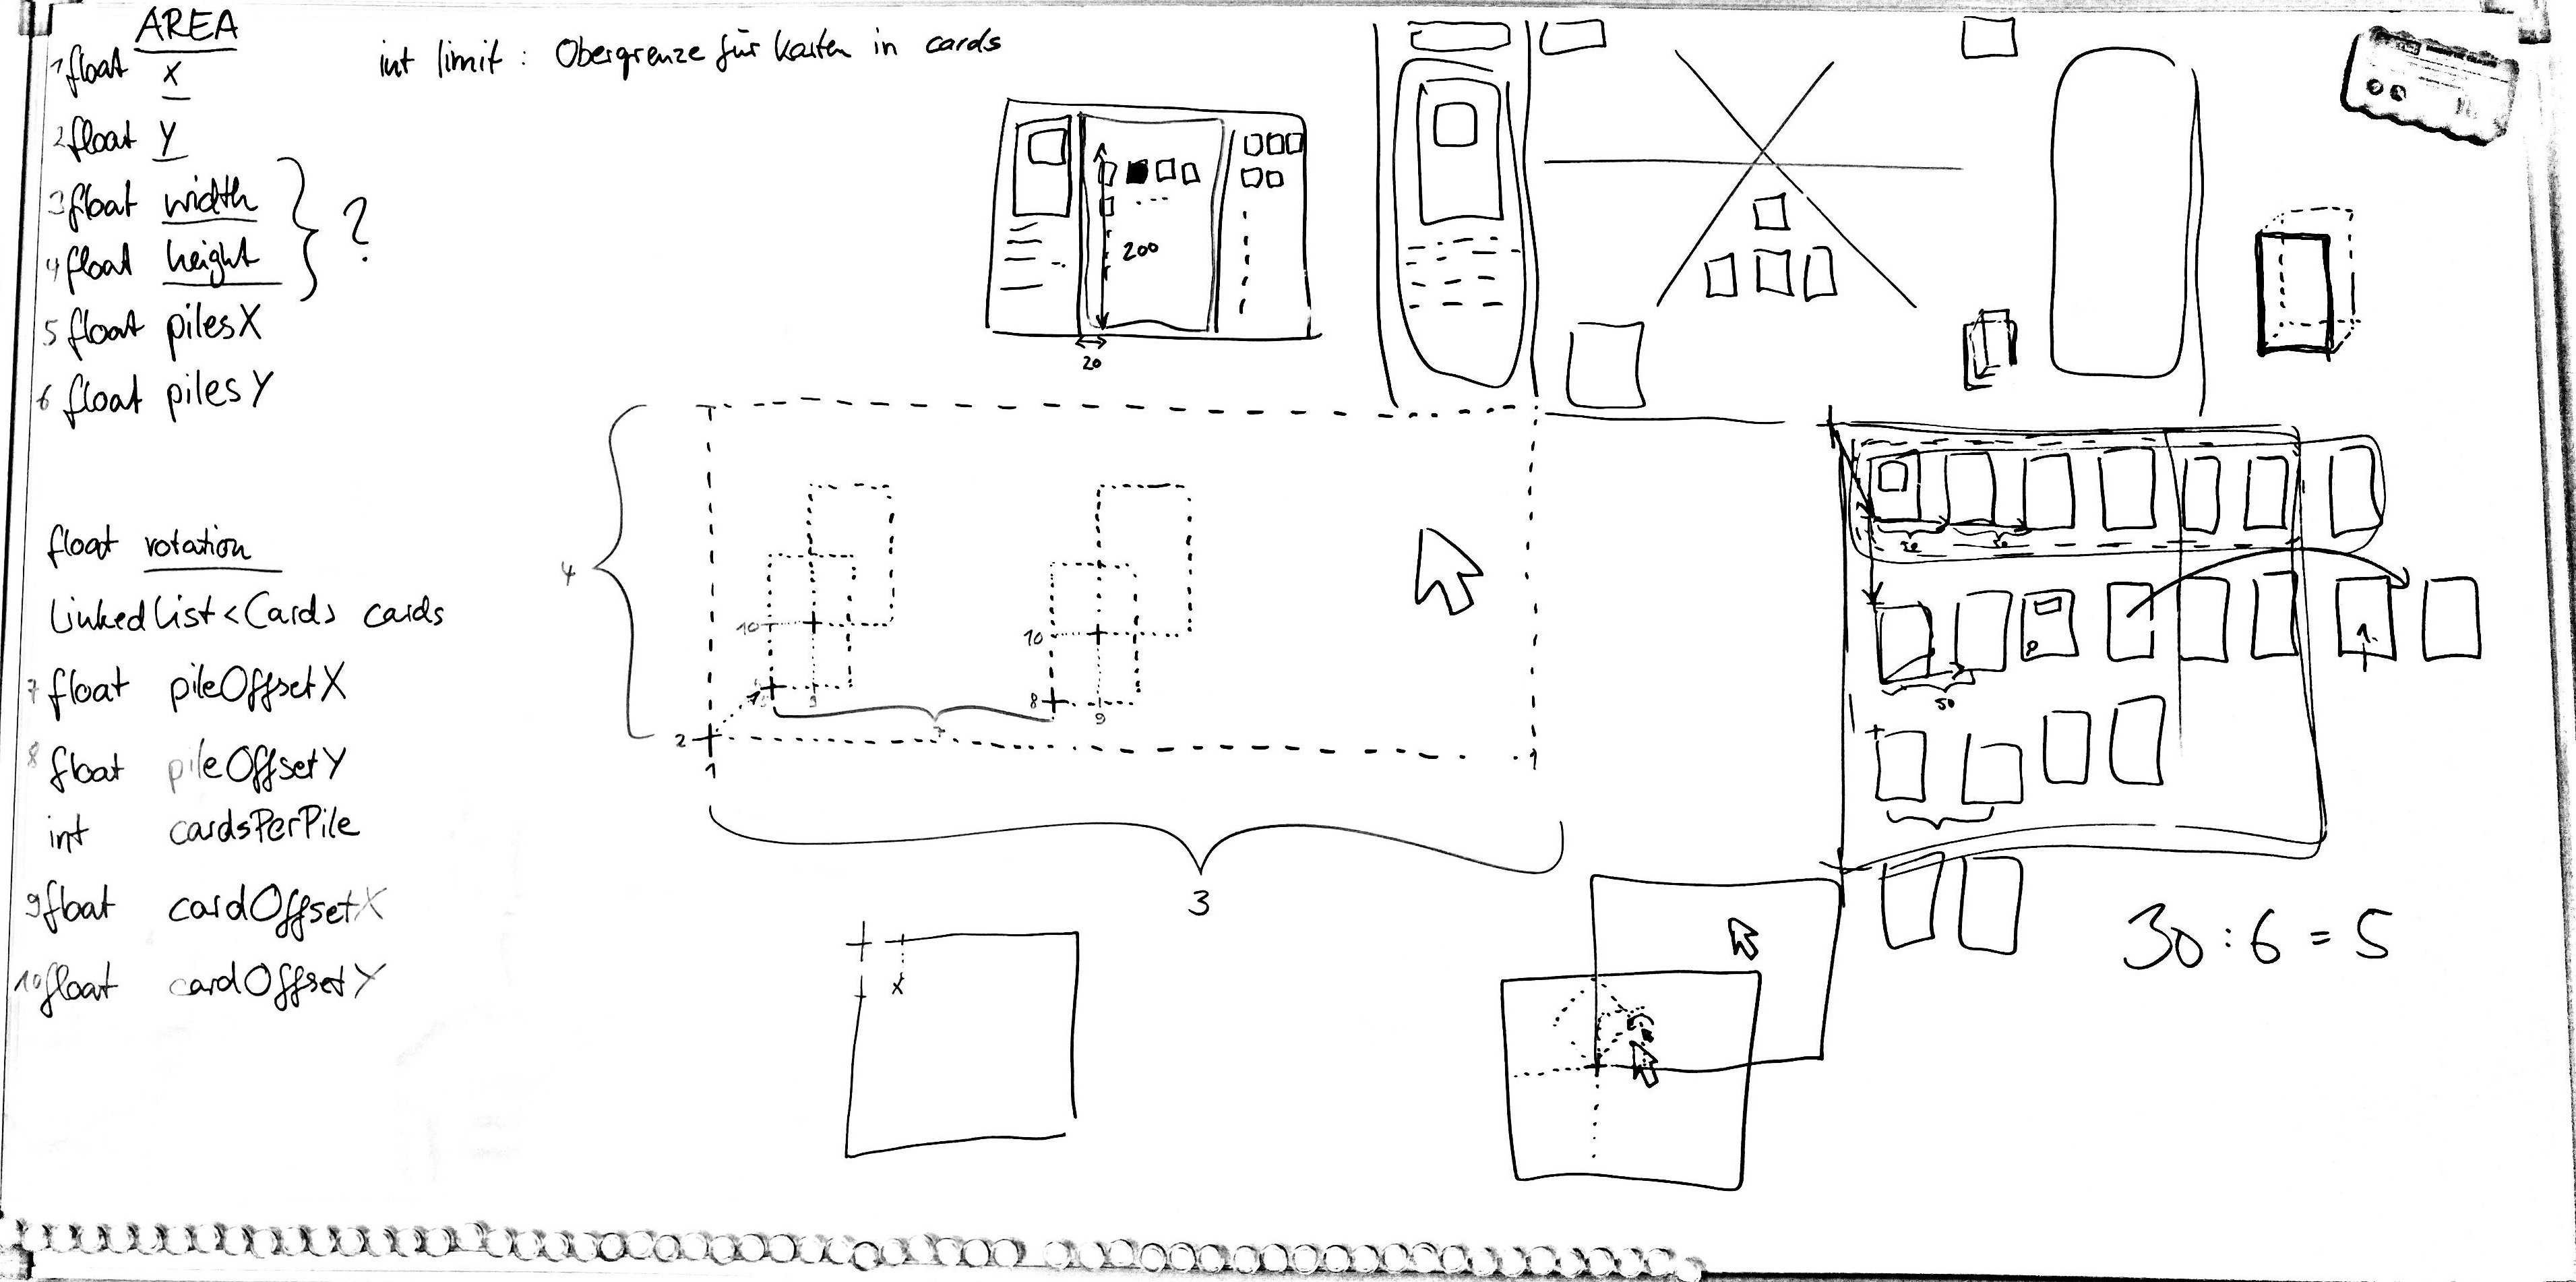
\includegraphics[width=1\textwidth]{../img/bild_fields.JPG}
\caption{Zeichnung: Fields}
\label{fig:Zeichung Fields}
\end{figure}

Jedes Field hat auch ein Kartenlimit, bei fast allen ist dieses 1. Nur beim Deck gibt es ein Limit von 40 Karten pro Field.
Im Field ist eine Update-Methode implementiert, die die Karten neu ordnet wenn eine Karte aus einem Field genommen wird. Die Methode macht logisch folgendes, die Methode itteriert durch die Karten des Piles durch, sie gibt jeder BattleCard ihre X- und Y-Werte neu bei jedem Update. So werden die Karten immer neu geordnet, wenn eine Karte zum Field hinzugefügt wird oder entfernt wird. Die Karten rücken also auf, damit keine Lücke entsteht.
Es gibt noch einige weitere Methoden in der Field-Klasse, diese werden folgend beschrieben.

\textbf{UpdateReadabilityOfBattleCard}
Diese Methode ruft die Methode getUncovered() von der BattleCard auf. Auf einem physikalischen Kartenspiel wäre das das Umdrehen der Karte von Rückseite auf Vorderseite. Wenn eine Karte z.B. auf dem Stapel liegt, ist diese umgedreht und nur die Rückseite der Karte ist sichtbar, welches die gleiche Textur bei allen Karten ist. Die getUncovered-Methode ändert die Textur der BattleCard von der Rücksteite-Textur zur Vorderseite Textur und ist jetzt sichtbar für den Spieler.

\begin{lstlisting}
protected void updateReadabilityOfBattleCard(BattleCard battleCard)
{
   battleCard.getUncovered();
}
\end{lstlisting}

\textbf{AddBattleCard}
Wie der Name schon sagt, wird hier eine Karte dem Field hinzugefügt. Unter der Haube passiert dennoch deutlich mehr. Es wird abgefragt, ob die Karte derzeit auf einem anderen Field liegt. Falls ja wird die Karte von diesem Field erst einmal entfernt. Außerdem wird die Existenz der Karte mit einer if-not-null-Kontrolle überprüft. Die Update-Methode wird am Ende aufgerufen.

\begin{lstlisting}
public void addBattleCard(BattleCard battleCardToAdd)
{
   Field currentField = FIELD_USER.giveBattleController().giveCurrentFieldOfBattleCard(battleCardToAdd);
   if (currentField != null) {
      currentField.removeCard(battleCardToAdd);
   }
   if (battleCardToAdd != null) {
      CARDS.add(battleCardToAdd);
   }
   update();
}
\end{lstlisting}

\textbf{AddBattleCards}
Man kann nicht nur einzelne Karten hinzufügen, sondern auch ArrayListen von Karten. Hier wird auch eine Abfrage gemacht, falls eine Karte schon auf einem anderen Feld ist, diese erst von diesem Feld zu entfernen. Für jede BattleCard von der ArrayList an Karten wird diese Abfrage gemacht und dann dem Field hinzugefügt.

\begin{lstlisting}
public void addBattleCards(ArrayList<BattleCard> battleCardsToAdd)
{
   for (BattleCard battleCard : battleCardsToAdd) {
      Field currentField = FIELD_USER.giveBattleController().giveCurrentFieldOfBattleCard(battleCard);
      if (currentField != null) {
         currentField.removeCard(battleCard);
      }
      CARDS.add(battleCard);
   }
   update();
}
\end{lstlisting}

\textbf{removeCard}
Von der ArrayList CARDS wird die BattleCard entfernt die als Parameter übergeben wird.

\begin{lstlisting}
private void removeCard(BattleCard cardToRemove)
{
   CARDS.remove(cardToRemove);
   update();
}
\end{lstlisting}

\textbf{PullCard}
Eine Karte wird anhand von ihrem index aus der ArrayList entfernt und dann zurückgegeben. Es gibt noch die Methode pullTopCard(), bei der der Index der Karte, die entfernt wird, einfach die ArrayList-Größe -1 ist. -1 weil Indices von 0 gezählt werden.

\begin{lstlisting}
public BattleCard pullCard(int index)
{
   if (CARDS.size() > 0 && CARDS.size() >= index && index >= 0) {
      BattleCard card = CARDS.get(index);
      removeCard(card);
      return card;
   } else {
      return null;
   }
}
public BattleCard pullTopCard()
{
   return pullCard(CARDS.size() - 1);
}
\end{lstlisting}

Es gibt noch 2 weitere Methoden und zwar shuffle(), die die ArrayList CARDS durchmischt und getPileSize(), die die Größe der CARDS ArrayList zurückgibt.

\begin{lstlisting}
public void shuffle()
{
   Collections.shuffle(CARDS);
}
public int getPileSize()
{
   return CARDS.size();
}
\end{lstlisting}

Am Anfang von jedem Spiel soll jedem Spieler Karten gegeben werden dies übernimmt giveCards().

\begin{lstlisting}
public ArrayList<BattleCard> giveCards()
{
   return new ArrayList<BattleCard>(CARDS);
}
\end{lstlisting}

\subsubsection{Laden und Speichern von Decks}
Ursprünglich war angedacht, dass ein Deckeditor umgesetzt werden soll. Dieser sollte dem Spieler ermöglichen, ein Karten-Deck nach seinen Wünschen zu gestalten, zu speichern und zu laden.  Als die Logik für das Feature "Effekte" jedoch vorerst nicht in das Gesamtprojekt eingefügt wurde, gab es nichts, anhand dessen sich die verschiedenen Kreaturen, Quartiere und Phenomene differenzierten. Daher machte auch darauf aufbauend eine Deck-Building mechanik erstmal keinen Sinn mehr. Trotz dessen wurde von Sebastian Beck eine einfache User-Klasse und ein SaveGameHandler implementiert. Die User-Klasse hielt die einzelnen Decks, während der SaveGameHandler als Utitlity-Klasse das Laden und Speichern zumindest backendseitig in ein Txt-File durchführte.

\subsection{Konzeptionelle und Organisatorische Aufgaben}
In diesem Abschnitt finden sich Aufgaben konzeptioneller sowie organisatorischer Natur, die sich mit dem Software-Entwicklungsprozess beschäftigt haben.

\subsubsection{Pflege eines schemenhaften Klassendiagramms}
Um die Struktur unseres Programmes grob zu visualisieren und so eine bessere Orientierung im Code zu ermöglichen sowie einen einheitlichen Wissensstand unter allen Beteiligten zu etablieren, erarbeitete und pflegte Felix Baumgarten ein Klassendiagramm.

Dieses half unter anderem, die Aufgabenverteilung mittels Git-Branches und die Kapselungsorganisation zu vereinfachen. Während der Arbeit am Projekt wurde das Diagramm an einem Whiteboard abgebildet und ergänzt, da Änderungen schnell umzusetzen waren und wir uns Einarbeitungszeit in komplexere digitale UML-Diagramme sparen wollten.
Eine Skizze des deutlich detaillierteren, da unter anderem mit Kardinalitäten ausgestatteten Klassendiagrams:
\begin{figure}[h]
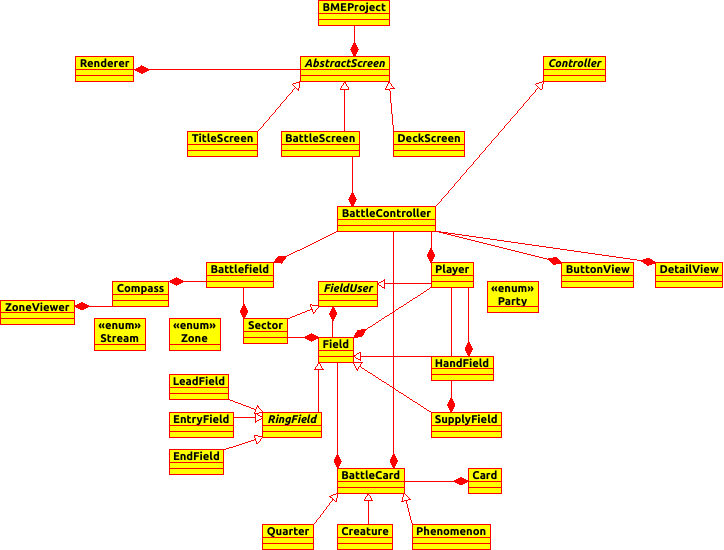
\includegraphics[width=1\textwidth]{../img/klassendiagramm.PNG}
\caption{Klassendiagramm Edwards Biotope}
\label{fig:Klassendiagramm_Edwards_Biotope}
\end{figure}
\subsection{Softwarequalität}
Hier finden sich die Neuerungen zum Thema Infrastruktur
\section{Gamedesign}
\subsection{Feinschliff: Fokus auf Stellungsspiel}
Bei Praxistests und in der Live Demo des letzten Semesters hat sich herausgestellt: Interessantestes Merkmal unserer Spielmechanik ist das Stellungsspiel der durch die Karten repräsentierten Spielobjekte.
Wo sich vergleichbare Trading Card Games stärker auf Zahlenschieberei konzentrieren (Verrechnen von Statuswerten, Sammeln von Zählmarken, Jonglieren mit Würfelergebnissen) orientiert sich unser Produkt am Prinzip des Brettspielklassikers Schach, dessen emergentes Potenzial ausschließlich aus der Vielfalt der Anordnungsmöglichkeiten seiner Figuren erwächst.
Die positive Resonanz zu diesem Umstand veranlasste Robert Sabo und Felix Baumgarten dazu, den Spielregeln einen letzten Feinschliff zu verpassen; im Zuge dessen die wenigen noch existenten Zahlen (Stärkewerte im oberen rechten Eck jeder Karte) über Bord zu werfen und das Stellungsspiel vollständig in den Mittelpunkt zu rücken. Zwar finden für konfrontative Auseinandersetzungen unter den Spielkarten noch immer Schadensberechnungen statt, doch basieren diese nicht mehr auf dem Vergleich individueller Statuswerte, sondern auf Kartentypen-abhängigen Eigenschaften:
\begin{itemize}
\item Jede Karte verfügt abhängig von ihrem Kartentyp über eine feste Anzahl an Trefferpunkten:
\begin{itemize}
\item Quartiere: 3 Trefferpunkte
\item Kreaturen: 2 Trefferpunkte
\item Phänomene: 1 Trefferpunkt
\end{itemize}
\item Ein Angriff reduziert die Trefferpunkte des Zieles stets um 1
\end{itemize}
Auf diese Weise wird das Regelwerk reduziert, die Kartengestaltung entschlackt und der Spielablauf vereinfacht – und gleichzeitig das Hauptaugenmerk unseres Gameplays unterstrichen.

\section{Grafik- und Sounddesign} 
\subsection{Video-Produktion}
Ein Trailer zu unserem Produkt (Videospiel), sollte erstellt werden. Dieses ca. 1 Minute Video soll im BB-Gebäude in einer Dauerschleife mit den anderen interdisziplinären Projekten aus unserem Studiengang an großen Monitoren gezeigt werden. Der Trailer soll einen kurzen Einblick zu unserem Videospiel geben. Dabei soll die Tonalität und Spezifizierung unseres Produkts (Cardgame) schnell erkennbar sein. Nach einer Ideensammlung einiger Teammitglieder in Form von Storyboards, wurde sich auf einen groben Aufbau geeinigt.
Um einen gewissen Überblick über den dramaturgischen Ablauf zu kriegen, hat Robert Sabo ein Videoscript zum Trailer angefertigt(Siehe Datei: Video-Teaser-Trailer/Videoscript.pdf). In diesem Script steht allgemein der Zeichenstil, die Schriftarten, Länge der Abschnitte und deren Einstellungen, sowie allgemeine Schnittkonventionen. Die Handlung wurde in mehrere Einstellungen aufgeteilt, die eine gewisse Dramaturgie unterstützen. Visuelle und auditive Angaben wurden hier auch festgelegt. Die jeweils drei Abschnitte wurden unter den Beteiligten aufgeteilt (Abschnitt 1: Manuela, Abschnitt 2: Robert, Abschnitt 3: Gabriel). Sämtliche Videosegmente wurden mit Adobe After Effekts realisiert. Die einzelnen Assets wurden mit Adobe Photoshop erstellt. Schlussendlich wurden die drei Abschnitte von allen Beteiligenten von Robert Sabo einheitlich in After Effekts zusammengeschnitten. Dabei war es wichtig die Tonalität gut herüberzubringen. Deshalb mussten Paar Abschnitte neu bzw. angepasst werden, um einheitlich zu wirken. Schlussendlich wurde die Datei im avi-Format gerendert. Da die Datei aber zu groß war, wurde sie mit Hilfe von Pia Korndörfer zu einem kleineren Format, mp4, komprimiert. Philadelphia Gauß hat noch extra für die Präsentation eine Trailer-Version mit Soundeffekten und Soundtrack erstellt, um auch einen passenden auditiven Eindruck des Videospiels für die Zuschauer zu geben.\\
Auf die einzelnen Abschnitte wird im Folgenden genauer eingegangen.

\subsubsection{Storyboard}
Für die Präsentation des Projekts musste ein kurzer Trailer angefertigt werden, der unser Projekt innerhalb einer Minute grob darstellt und dem Zuschauer Lust auf unser Spiel macht. Um erste Anregungen zu sammeln, wurde sich zusammengesetzt und Ideen miteinander ausgetauscht. Im Anschluss bekamen Gabriel, Pamela, Cigdem und Manuela die Aufgabe, Storyboards anzufertigen. Somit sollten die gesammelten Ideen veranschaulicht werden.
Ein Storyboard ist eine Art visuelles Drehbuch, in dem Abläufe von Szenen konzipiert werden. Es kann skizziert, aber auch collagiert sein. Innerhalb des Storyboards können Kameraschnitte, Bewegungsanweisungen, Überblendungen und auditive Ansagen festgehalten werden.
Der Trailer muss den Zuschauer in die Unterwasserwelt von EDWARDS BIOTOPE eintauchen lassen und sowohl einen Vorgeschmack für die Hintergrundgeschichte als auch eine kurze Sicht auf die Spielmechanik bieten. Dennoch sollte eine Länge von einer Minute nicht überschritten werden. Genau das galt es bei der Erstellung der Storyboards zu beachten. Das entsprechende Storyboard ist im Anhang beigefügt. \\Letztendlich wurde sich nicht für eines der Storyboards entschieden, sondern es wurden die verschiedenen Umsetzungen miteinander kombiniert. Dies ergab schließlich die Vorgabe für unseren Trailer, der dann von Robert und Pia umgesetzt wurde. \\
In unserem Gameplay-Trailer sollte der grobe Spielablauf dargestellt werden. Als Programm wurde Adobe After Effects CC verwendet.
Wie bereits Eingangs beschrieben, wurden für das Video mehrere Storyboards angefertigt. Hierzu ein Auszug in Abbildung \ref{fig:Storyboard: Spielfeld}

\begin{figure}[h]
\centering
 \subfloat[Storyboard: Spielfeld 1]{{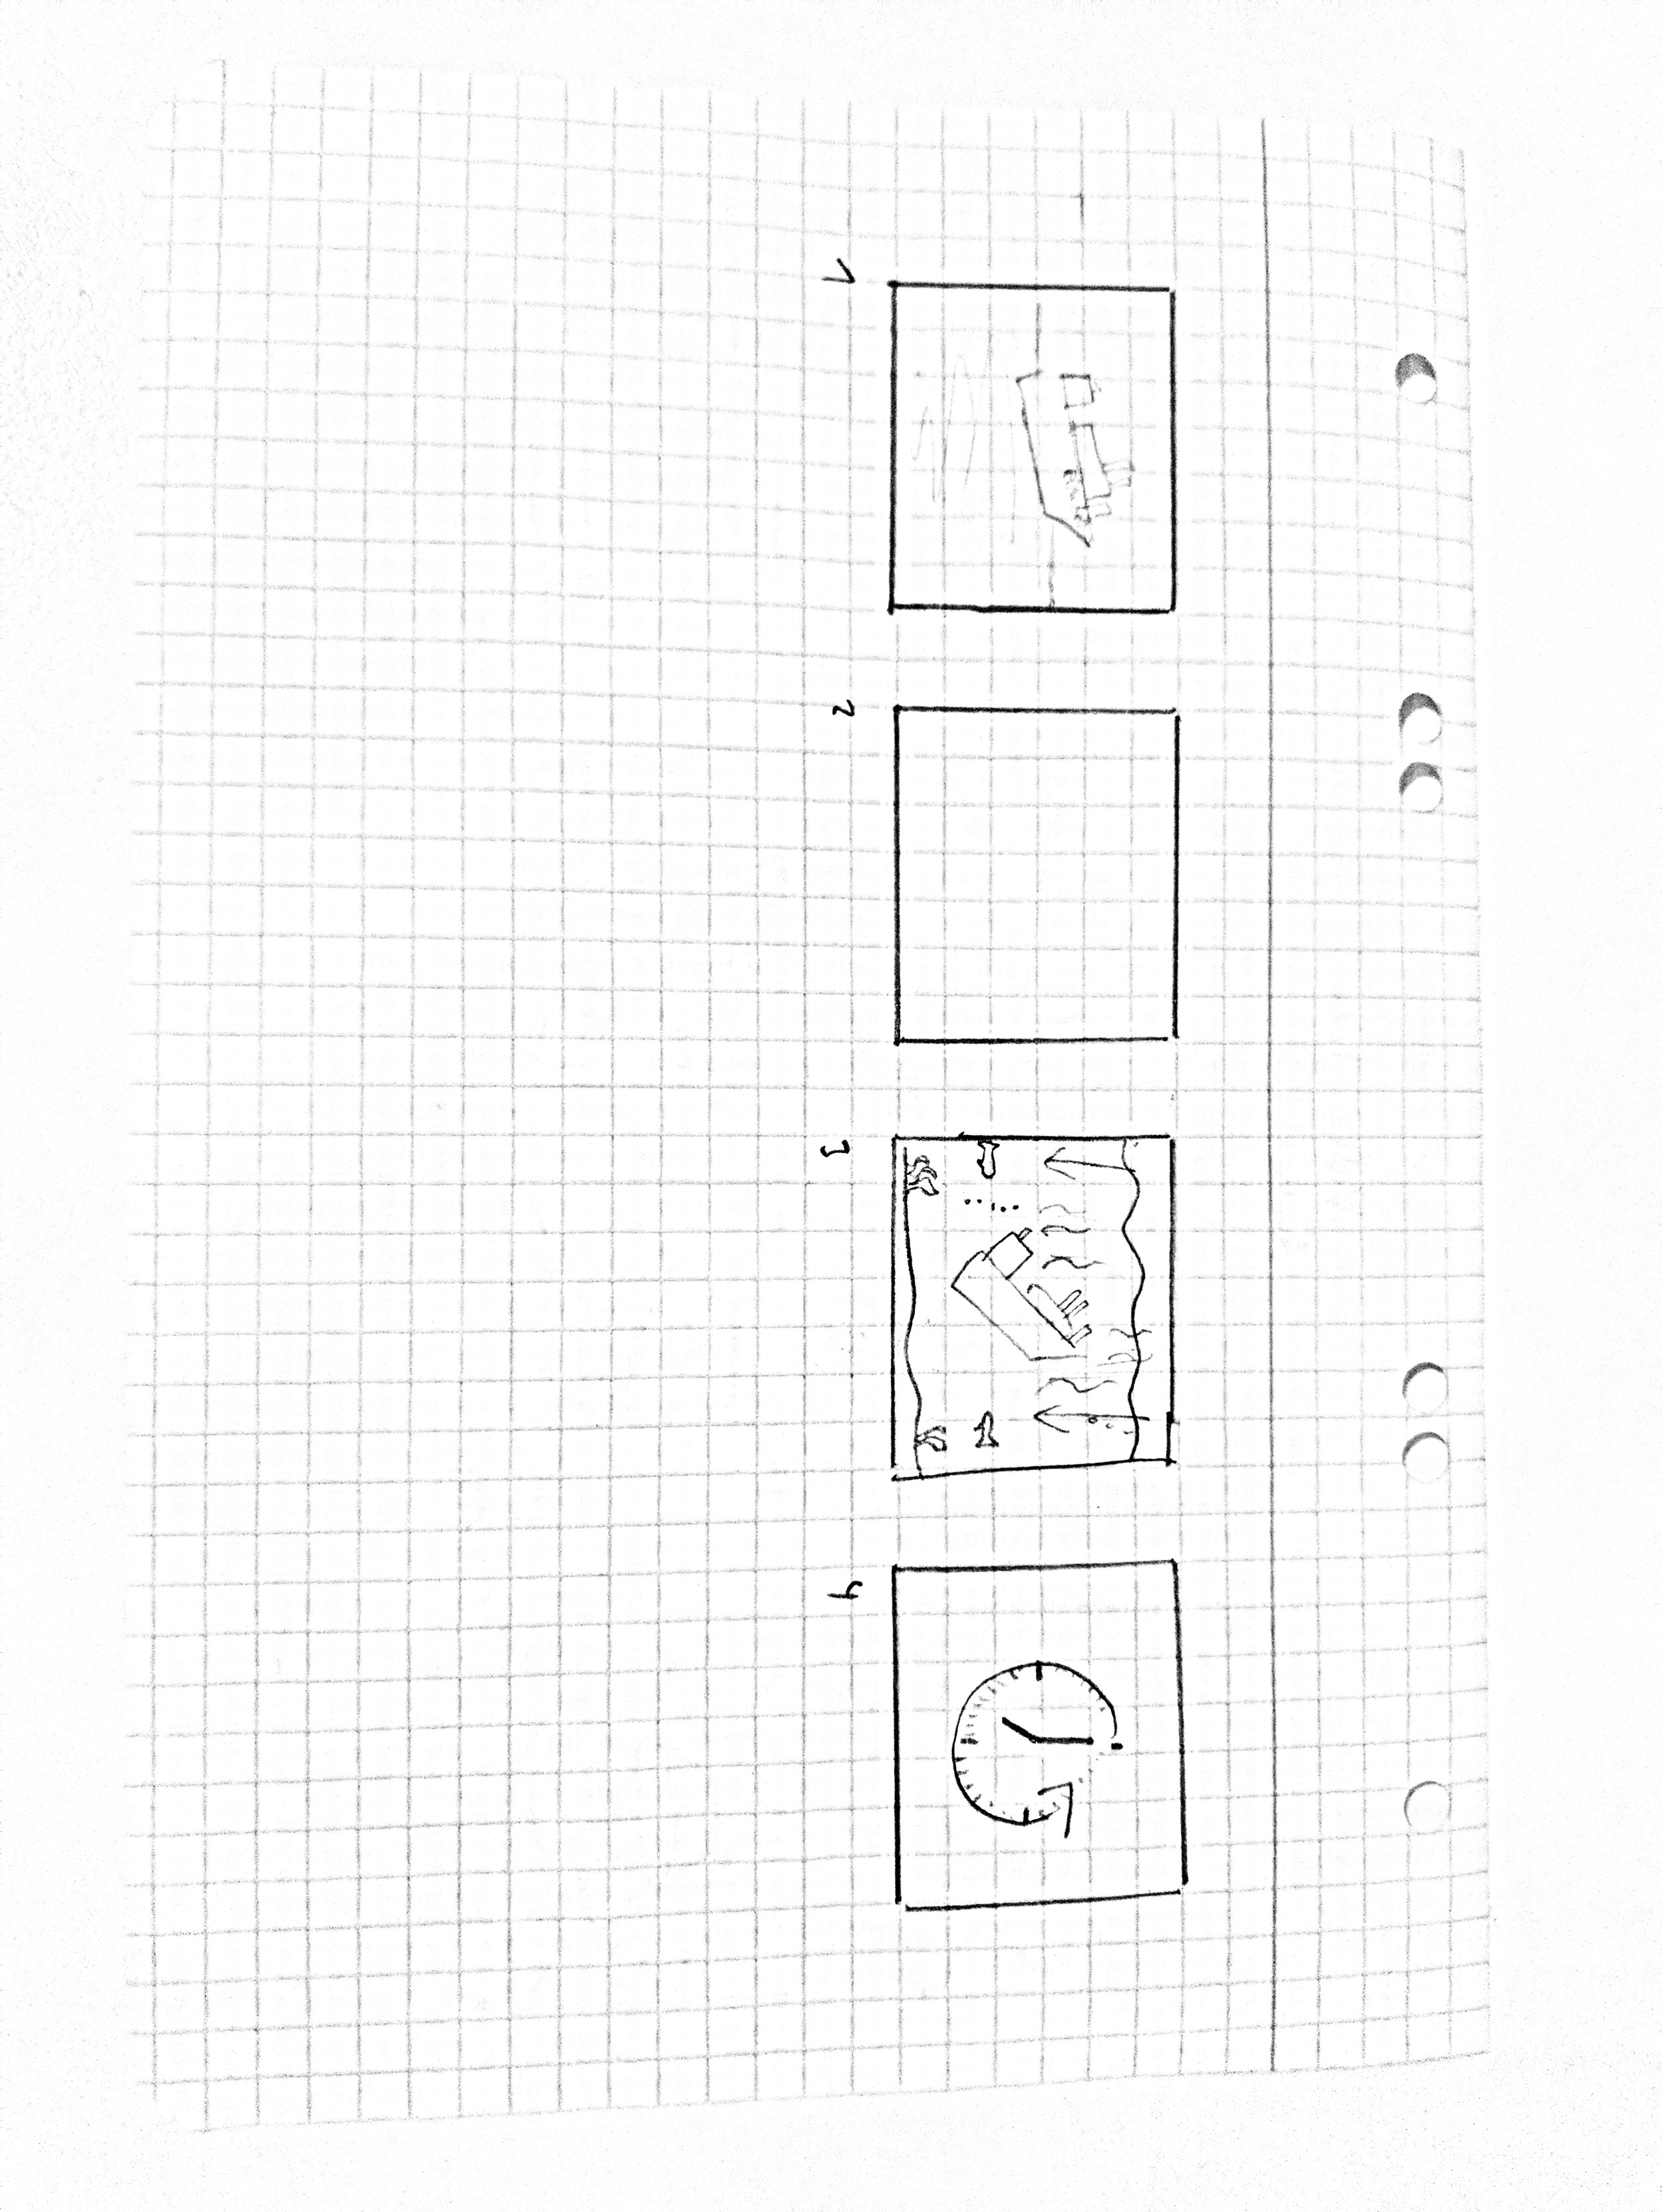
\includegraphics[width=4cm]{../img/storyboards/storyboard_1.JPG} }}
\qquad
 \subfloat[Storyboard: Spielfeld 2]{{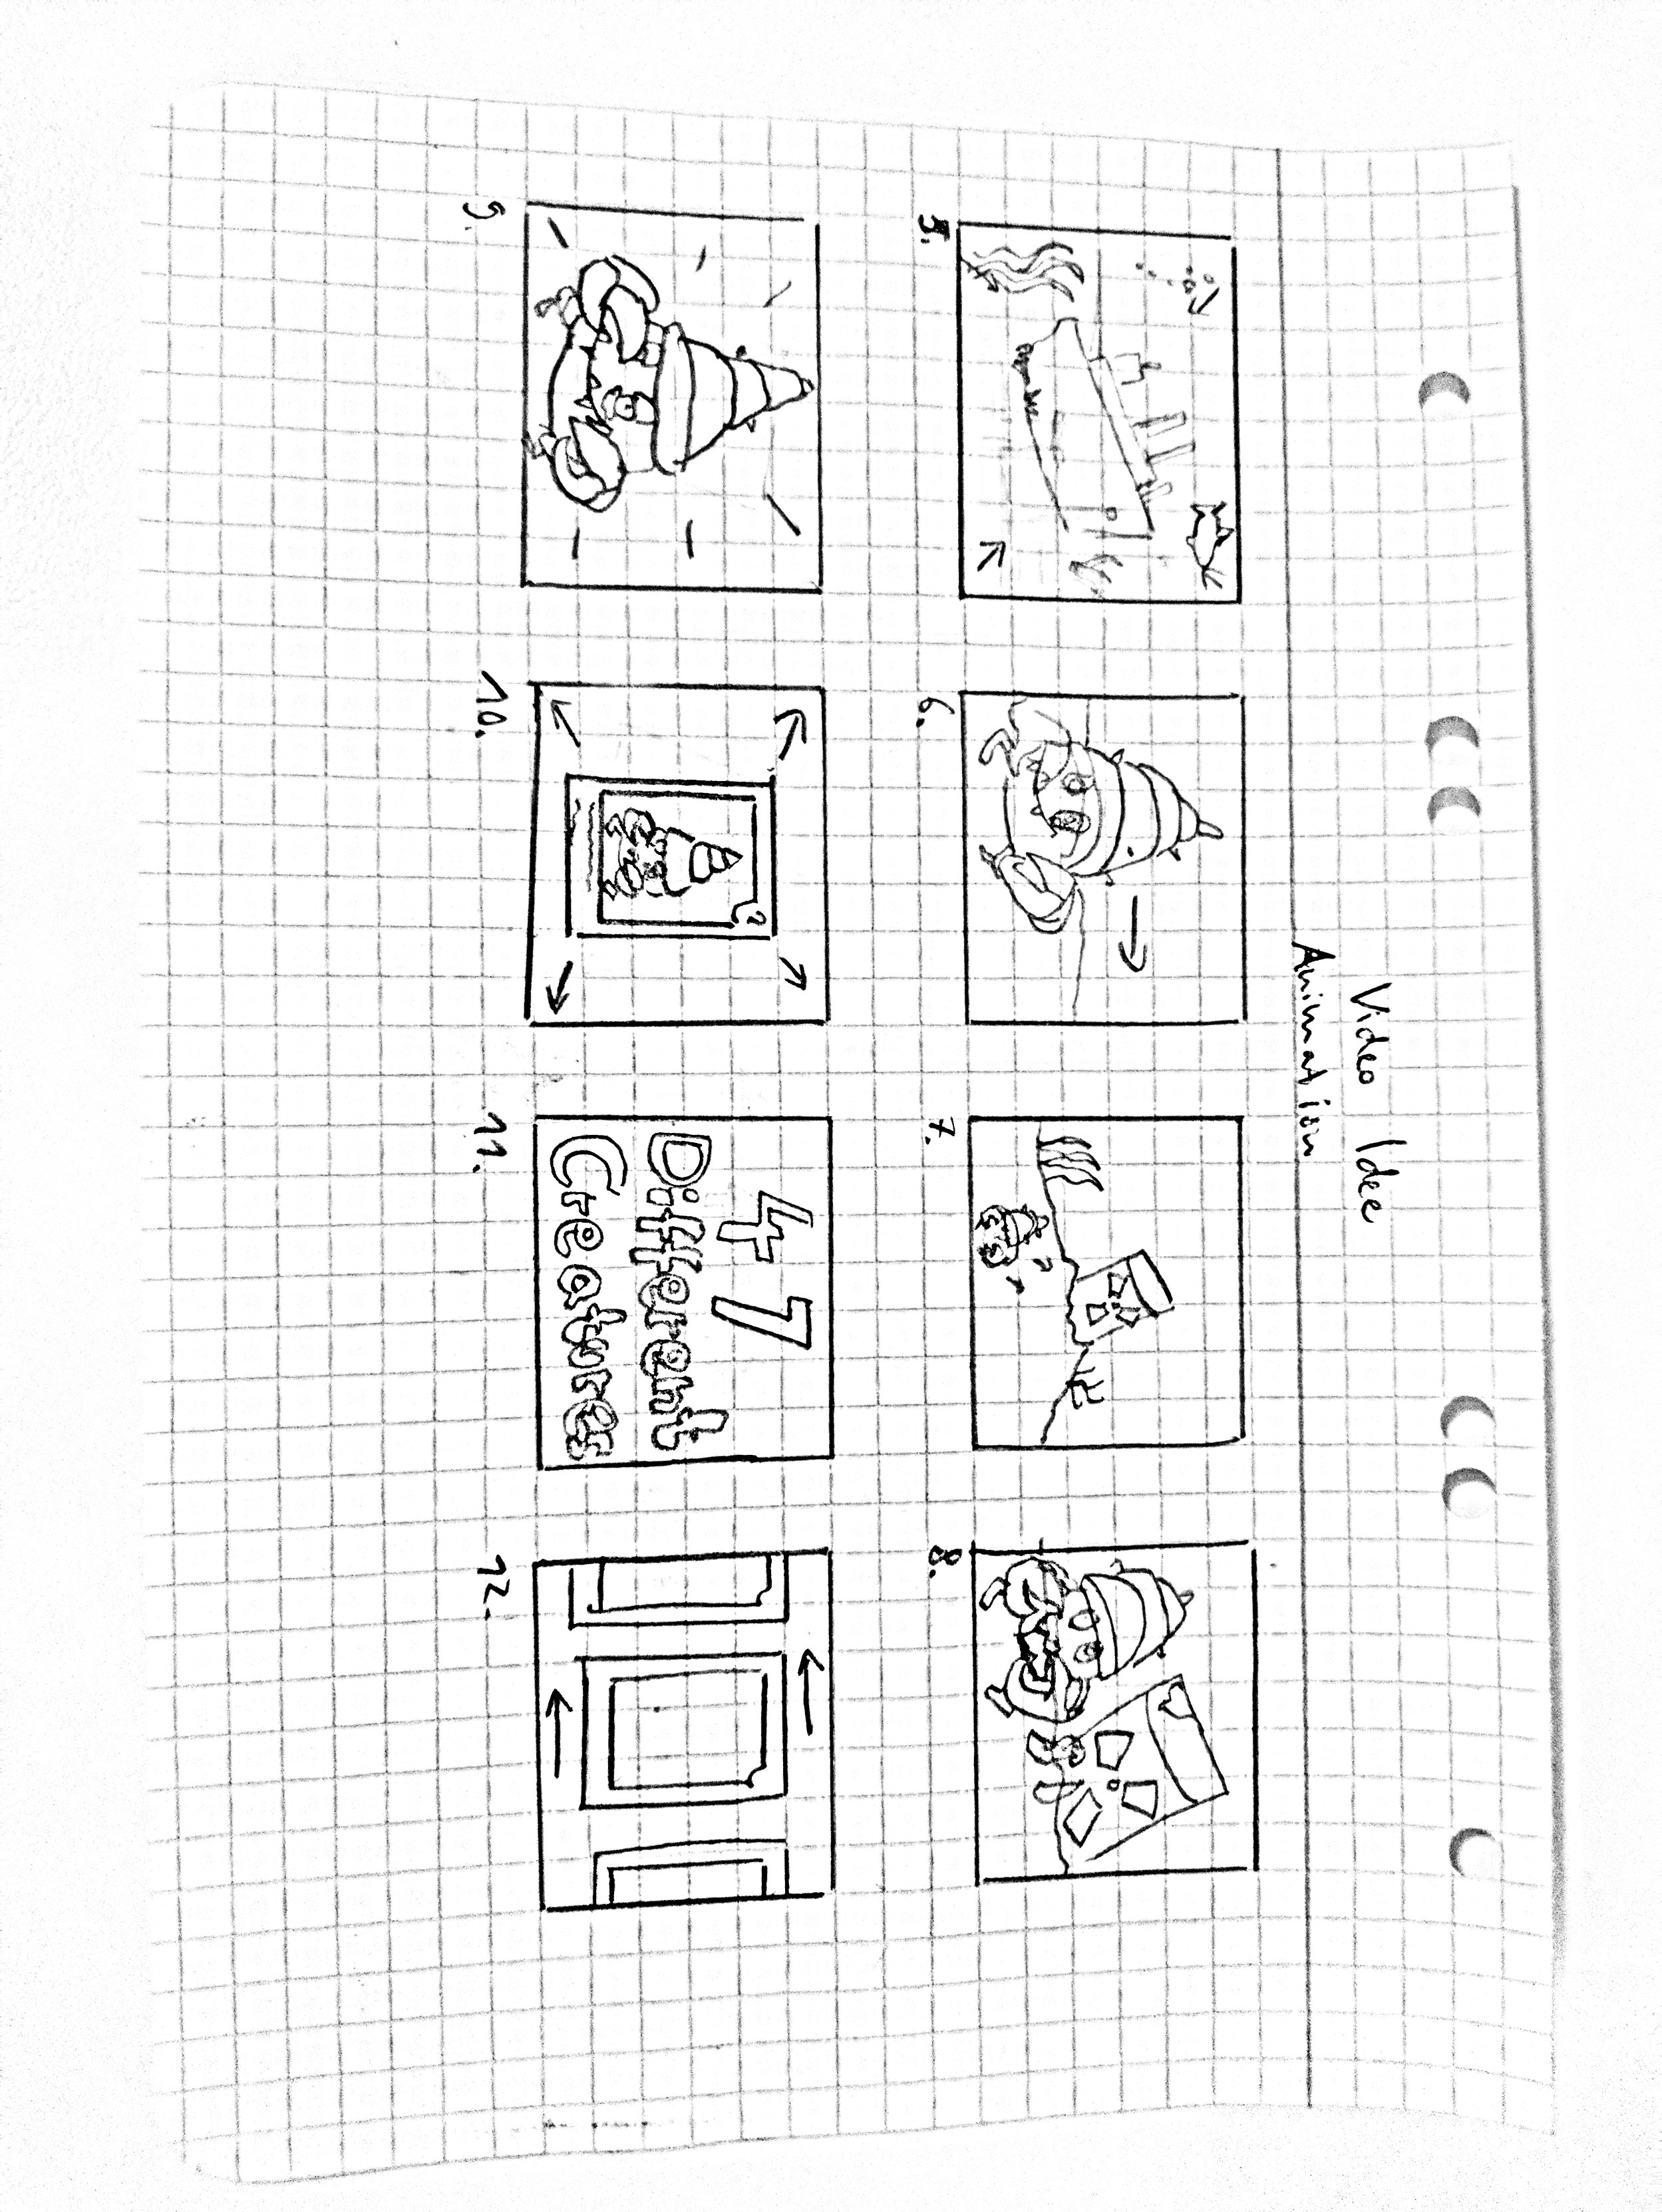
\includegraphics[width=4cm]{../img/storyboards/storyboard_2.JPG} }}
\qquad
 \subfloat[Storyboard: Spielfeld 3]{{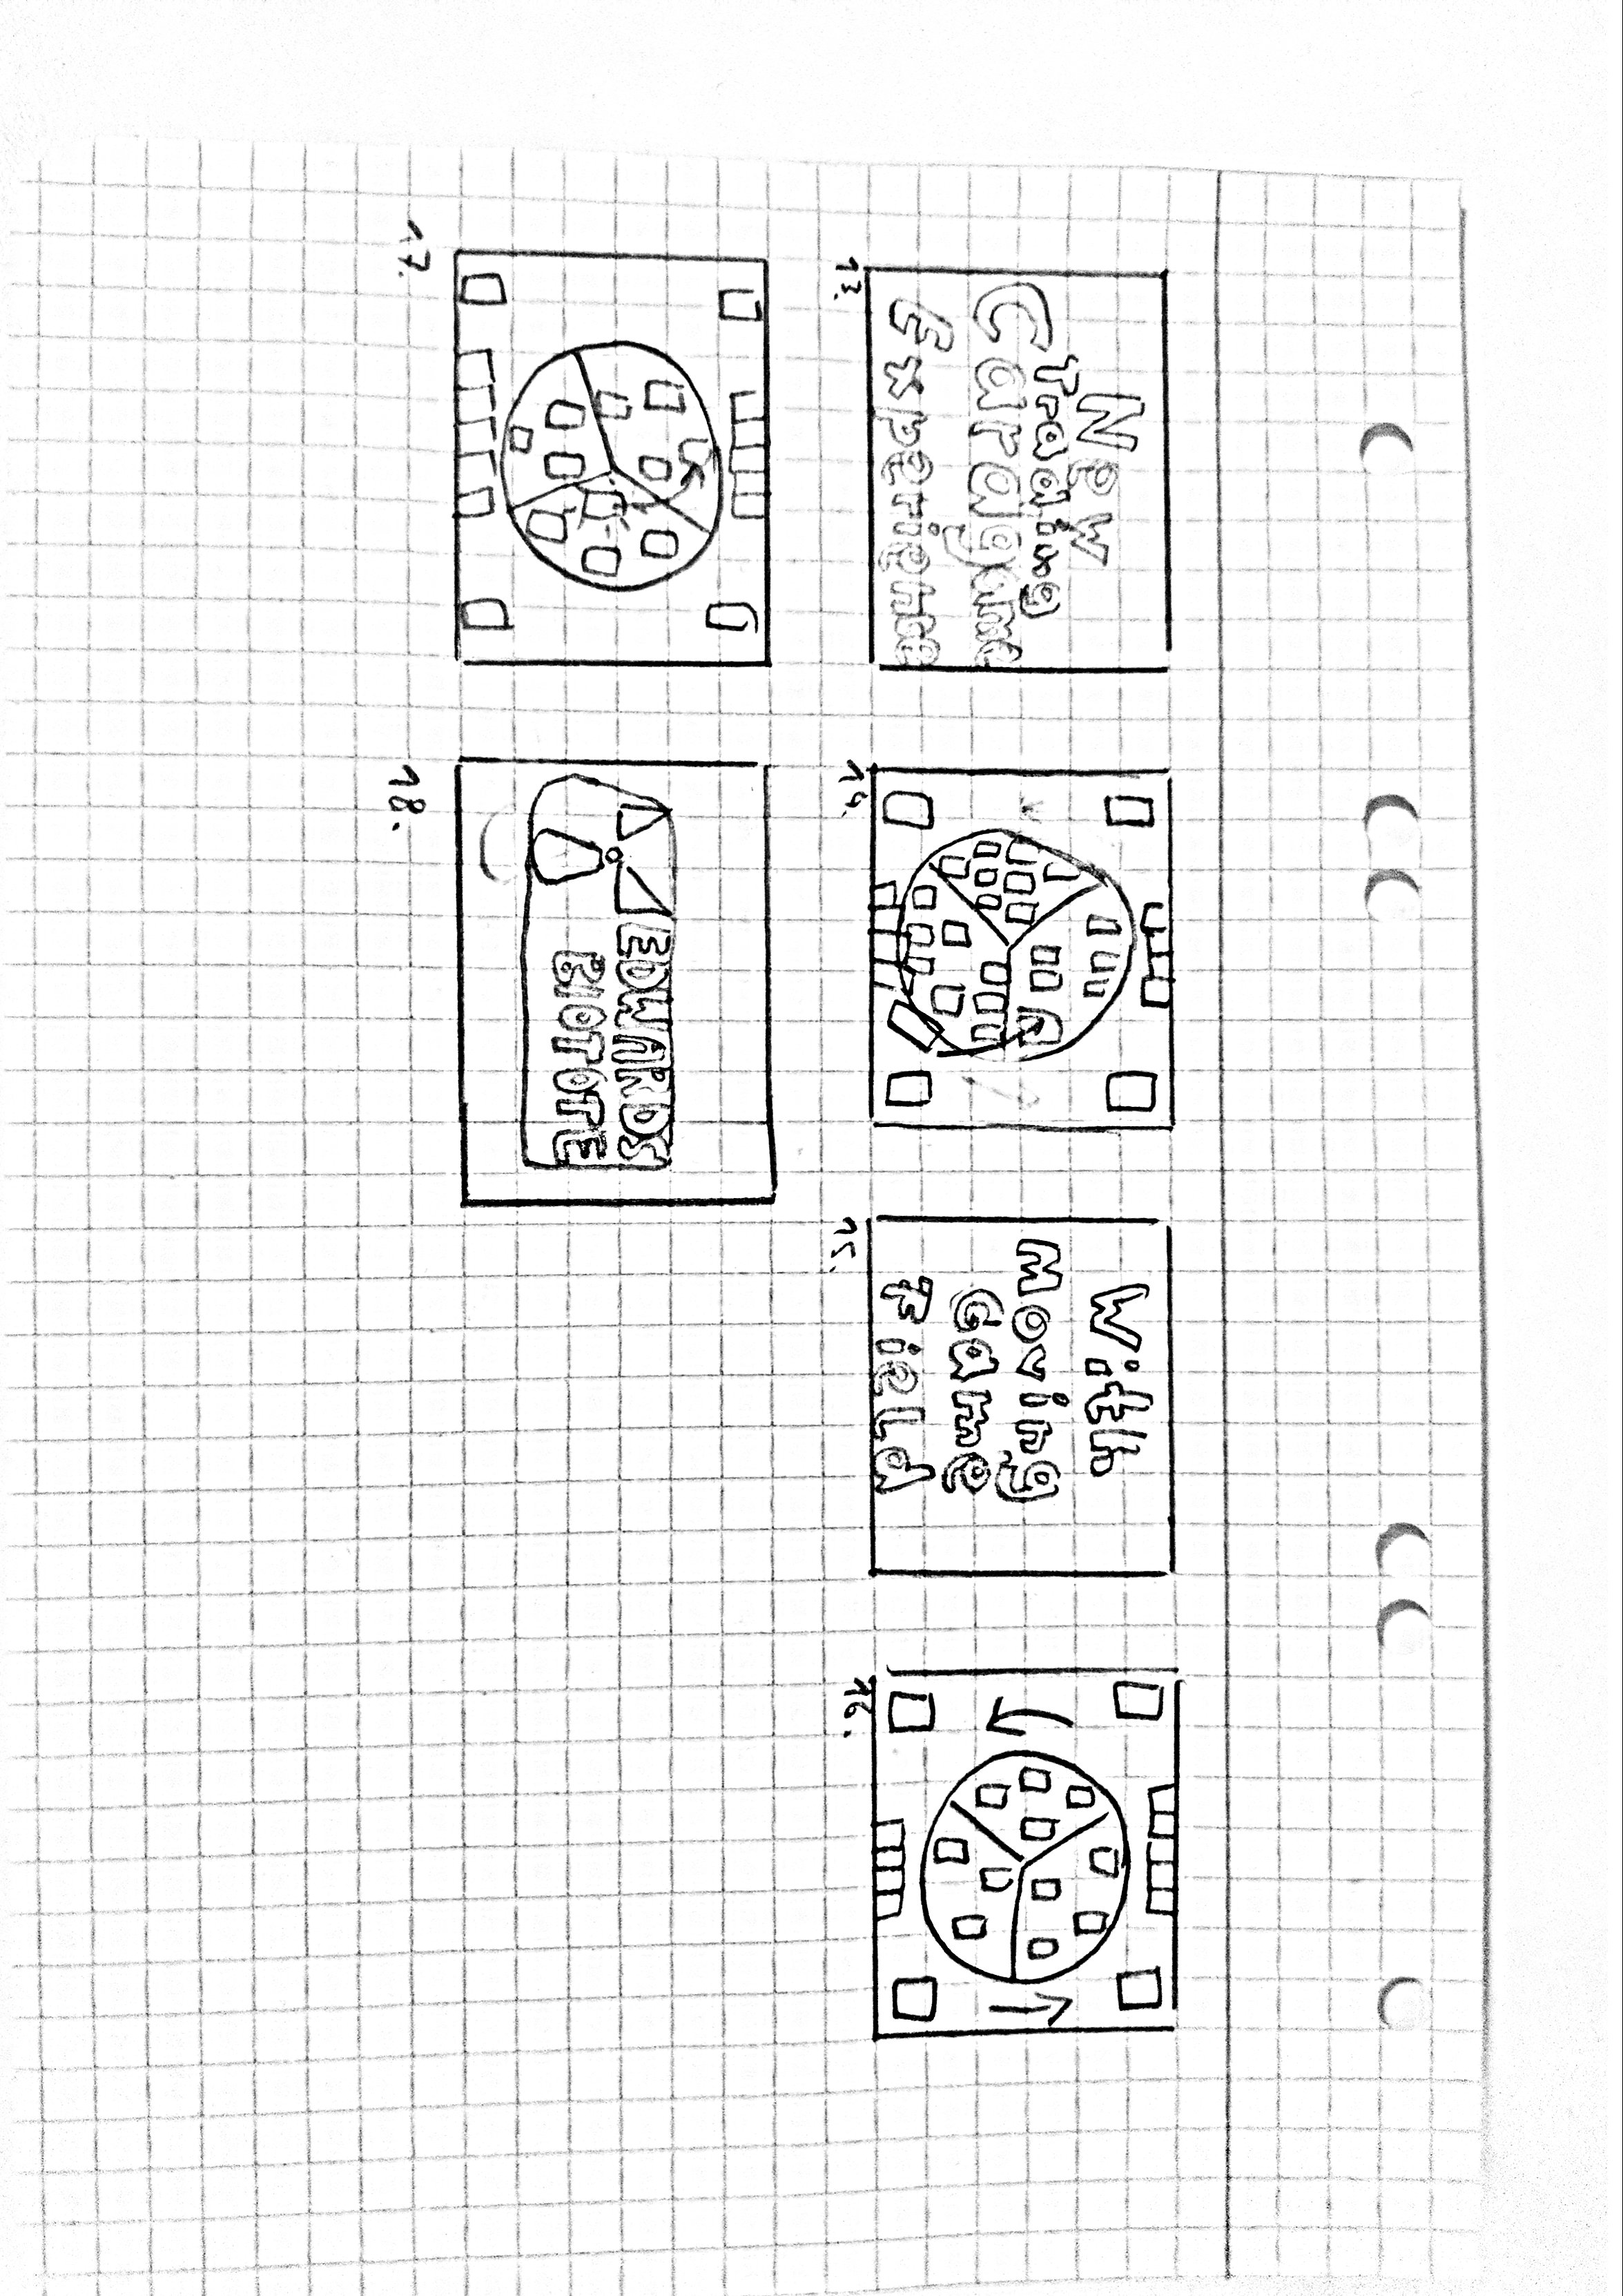
\includegraphics[width=4cm]{../img/storyboards/storyboard_3.JPG} }}
\caption{Storyboard: Spielfeld}%
 \label{fig:Storyboard: Spielfeld}%
\end{figure}
Nach einiger Überlegung wurde sich auf ein Storyboard geeinigt und den Trailer in 3 Abschnitte aufgeteilt, für die jeweils eine Person zuständig war. Abschnitt 1 ist die Vorgeschichte/Intro, Abschnitt 2 die Verwandlung der Kreaturen in mutierte Monster und Abschnitt 3 Ingame-Gameplay. Hier wird die Arbeit an Abschnitt 3 beschrieben.\\
In Abschnitt 3 soll das Gameplay des Spiels gezeigt werden und zwar so nah am Endprodukt wie möglich. Dies war nicht sehr leicht, weil manche Ideen zum Gameplay noch nicht absolut feststanden. Die Idee war es die Grundfunktionen des Gameplays zu zeigen wie z.B. Farbrad drehen, Strömungsrichtung, Zonenaktivierung und einen ausgeführten Angriff. In dieser weise könnte ein Spielzug eines Spielers aussehen und es war wichtig diesen Ablauf einzuhalten. Zum Animieren wurden hauptsächlich die original Spiele-Assets verwendet, wobei bei den Spezialeffekten und der Seitenleiste die Original-Buttons noch nicht feststanden.
\begin{figure}
\centering
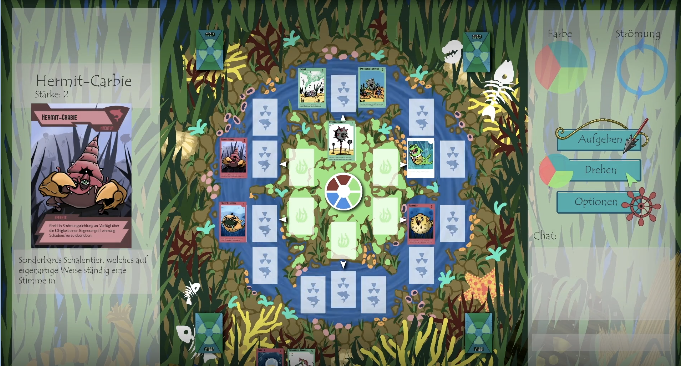
\includegraphics[width=0.8\textwidth]{../img/video_spielfeld.PNG}
\caption{Darstellung des Spielfelds im Trailer}
\label{fig:Videodarstellung Spielfeld}
\end{figure}
In Adobe After Effects wird anhand von Keyframes animiert. AE ist ein Compositing-Tool, das in Ebenen funktioniert, anders als Nuke(Compositing-Programm), das in Nodes aufgebaut wird.
Pro Ebene ist ein Asset eingefügt. Jedes Asset lässt sich beliebig drehen, vergrößern, transparent machen und bewegen. Diese ganzen Parameter lassen sich auch über Keyframes definieren. Keyframes sind von der Zeitleiste abhängig, d.h. an dem Zeitpunkt an dem ein Keyframe ist, müssen die eingestellten Parameter angewendet sein. Von einem Keyframe zum nächsten wird diese Änderung aber interpoliert dargestellt, wodurch eine gleichmäßige Änderung im Video zu sehen ist.
Dieser Workflow ist deutlich einfacher als Gameplay aufzunehmen oder vor allem Bild für Bild selber zu bearbeiten.

\subsubsection{Einarbeitung in After Effects}
Zunächst einmal erfolgte eine intensive Einarbeitungsphase mit dem Programm „After Effects“. Dabei waren sehr gute Youtube Tutorials eine große Unterstützung. 
Das Resultat von dem ersten Testvideo schaut wie folgt aus: 
\begin{figure}[h]
\centering
 \subfloat[Screenshot: After Effects 1]{{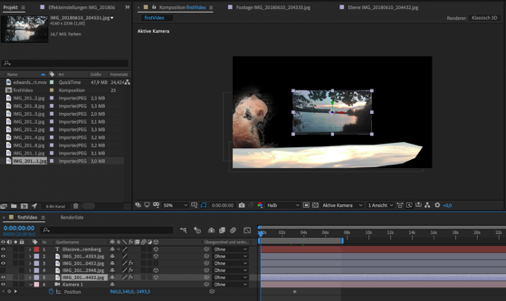
\includegraphics[width=5cm]{../img/screenshot_aftereffects_1.PNG} }}
\qquad
 \subfloat[Screenshot: After Effects 2]{{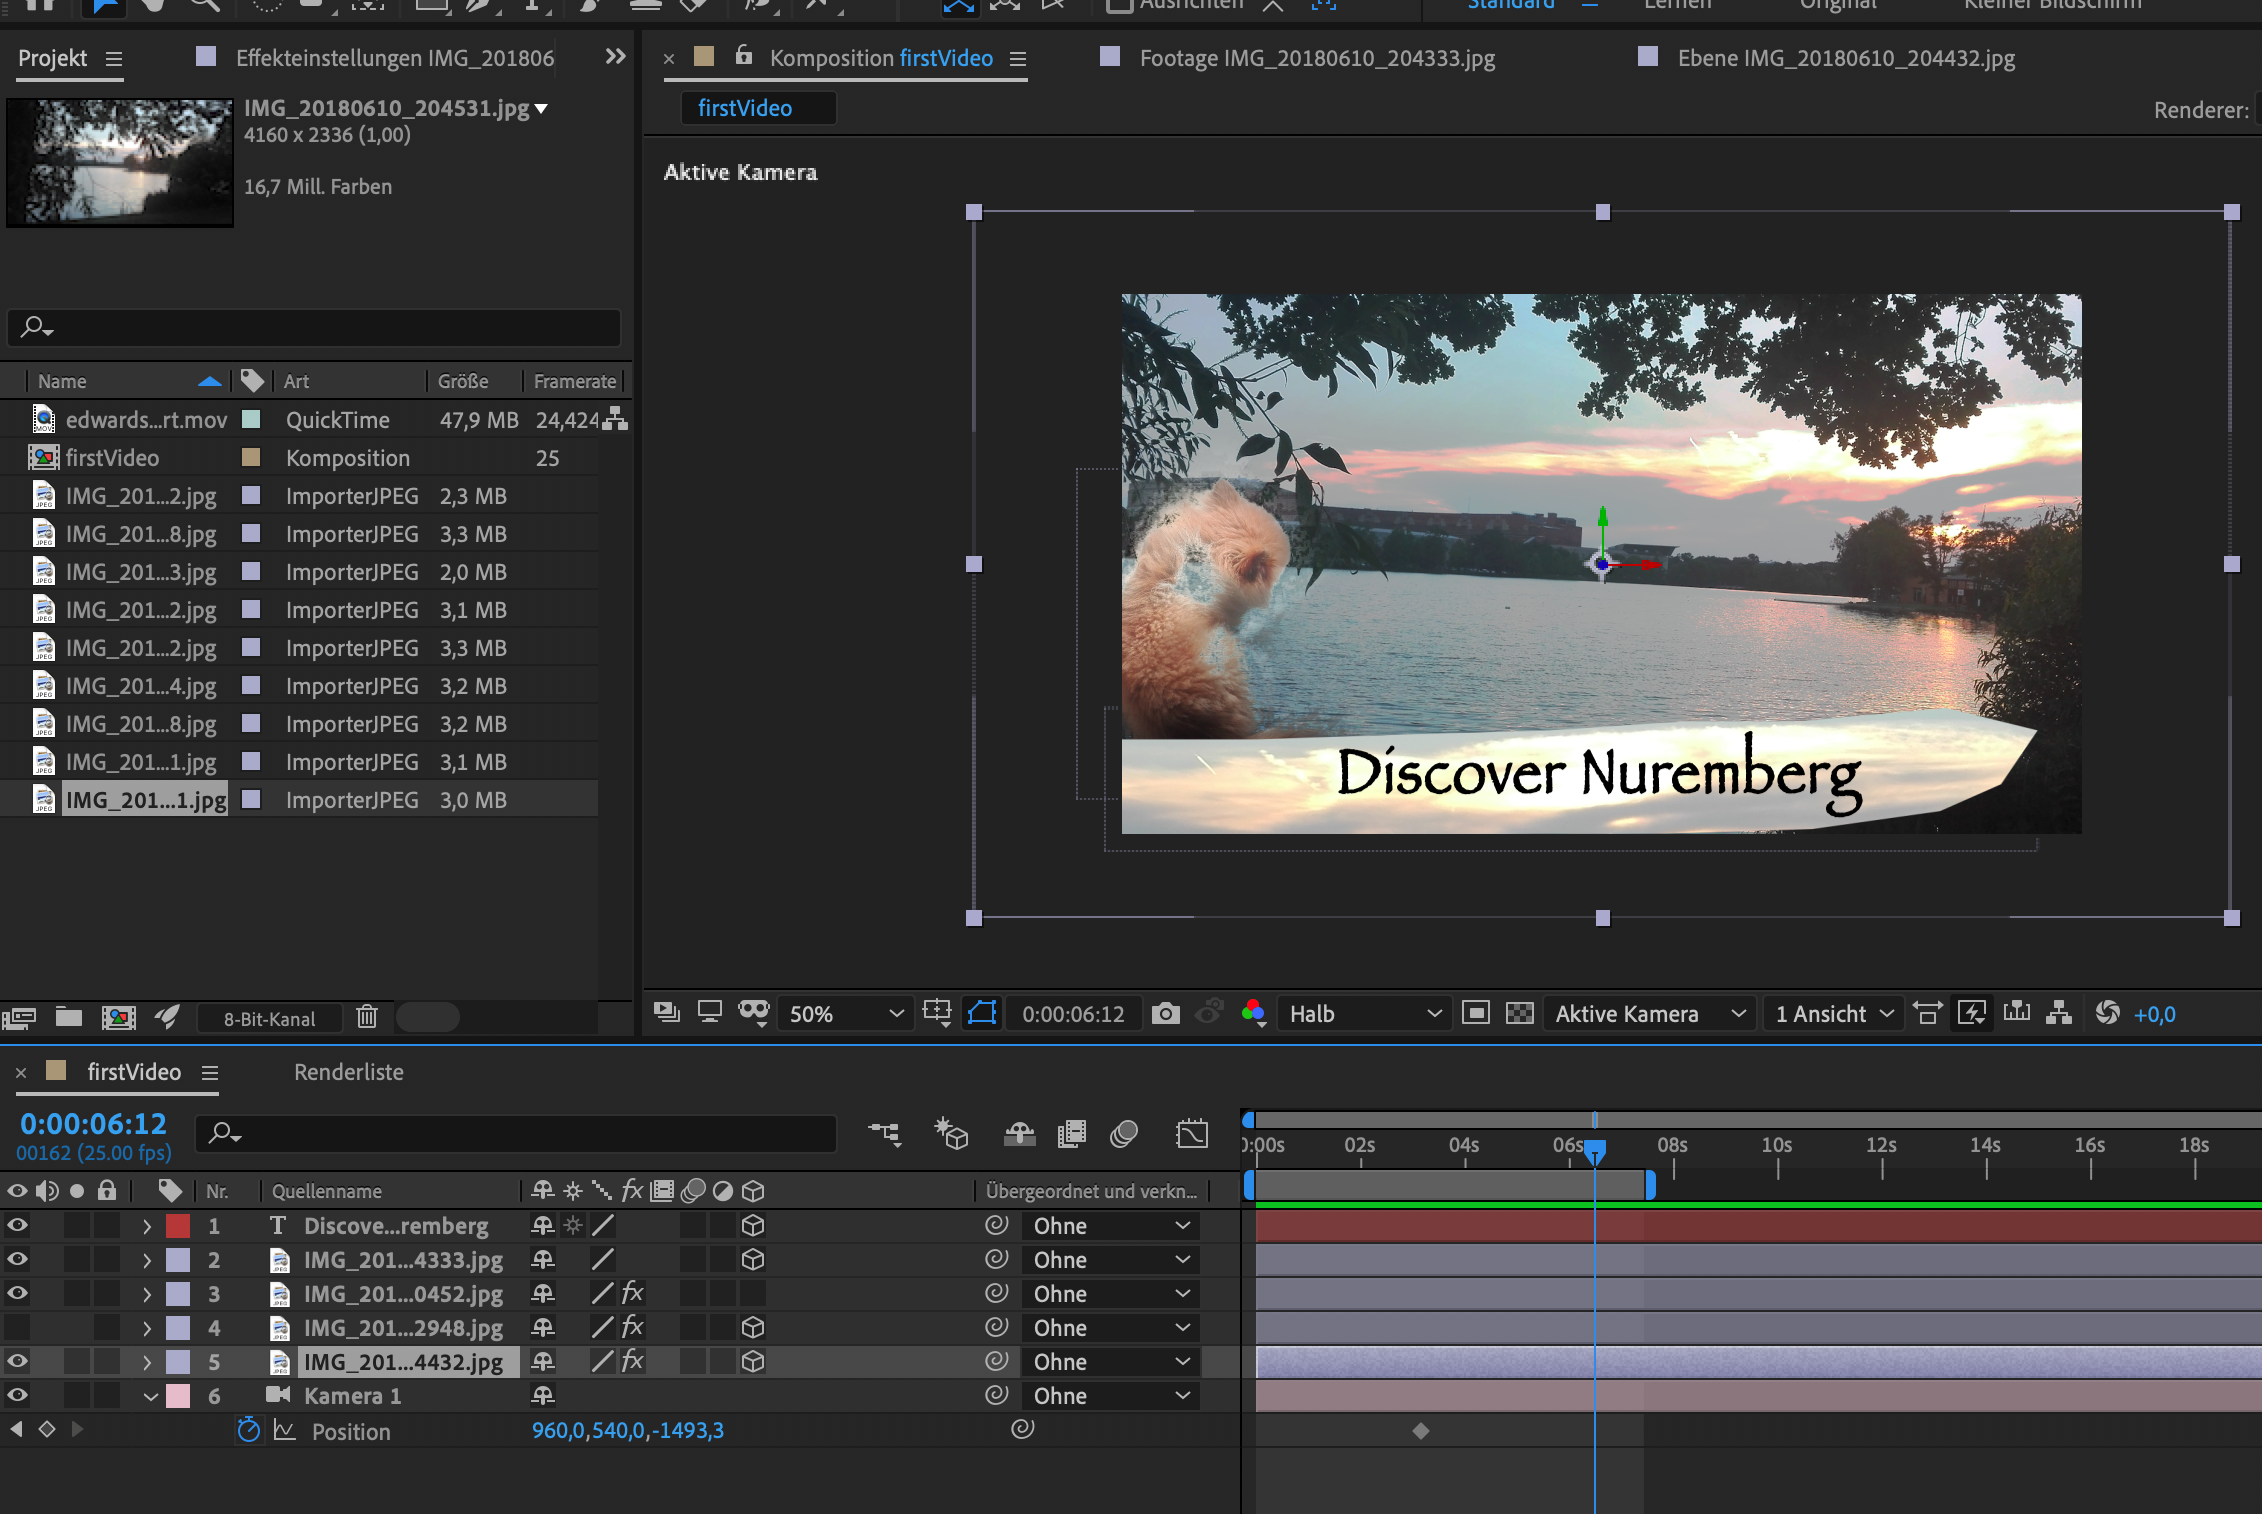
\includegraphics[width=5cm]{../img/screenshot_aftereffects_2.PNG} }}
\caption{Screenshots After Effects}%
 \label{fig:Screenshots After Effect}%
\end{figure}
Hierbei wurden Bilder freigestellt, ein Bild und der Titel animiert.  \cite{After Effects Einsteigertutorial}, \cite{How to Create Cartoon Animation}, \cite{After Effects Tutorial: Logo Animations}

\subsubsection{Produktion Video Intro}
Für einen Einstieg in die Geschichtsthematik des Spieles wurde der Betrachter mittels einer Kamerafahrt über das Meer an den eigentlichen Veranstaltungsort mitgenommen.
Dafür wurde ein längliches Bild angefertigt, das in AfterEffects zu einer Komposition hinzugefügt wurde. Anschließend wurde eine neue “Kamera” erstellt und die 3D-Funktionen der Kompositionsebene aktiviert. Nun mussten nur noch zwei Keyframes gewählt werden, den Startkeyframe am unteren, sowie den Endkeyframe am oberen Ende des Bildes.
Da Wasser, noch spezifischer gesehen Wellenbewegungen, sehr komplex zu animieren sind, wurde für die nächste Szene eine Wellenreihe in Adobe Animate angefertigt. Das Programm ermöglichte es die “Meereszacken” durch Anfertigung und Abspielen verschiedenster Frames zum Rotieren zu bringen. In After Effects importiert ergaben diese hintereinander liegenden Reihen in unterschiedlicher Ablaufgeschwindigkeit die Illusion einer sich bewegenden Meeresoberfläche. 
Das angefertigte Schiff musste jetzt an die Bewegungen der vordersten Welle angepasst werden. Diese Bildverschiebung kann in After Effects durch das Verändern der Position als auch Rotation sowie durch das Setzen mehrerer Keyframes (siehe Abbildung x) visualisiert werden. Auch der Hintergrund sowie der Blitz musste vorerst angefertigt und implementiert werden. Um das Aufleuchten des Blitzes naturgetreuer darzustellen, wurde seine Darstellung zwischen Erscheinen und Verschwinden noch verdoppelt. 
\begin{figure}
\centering
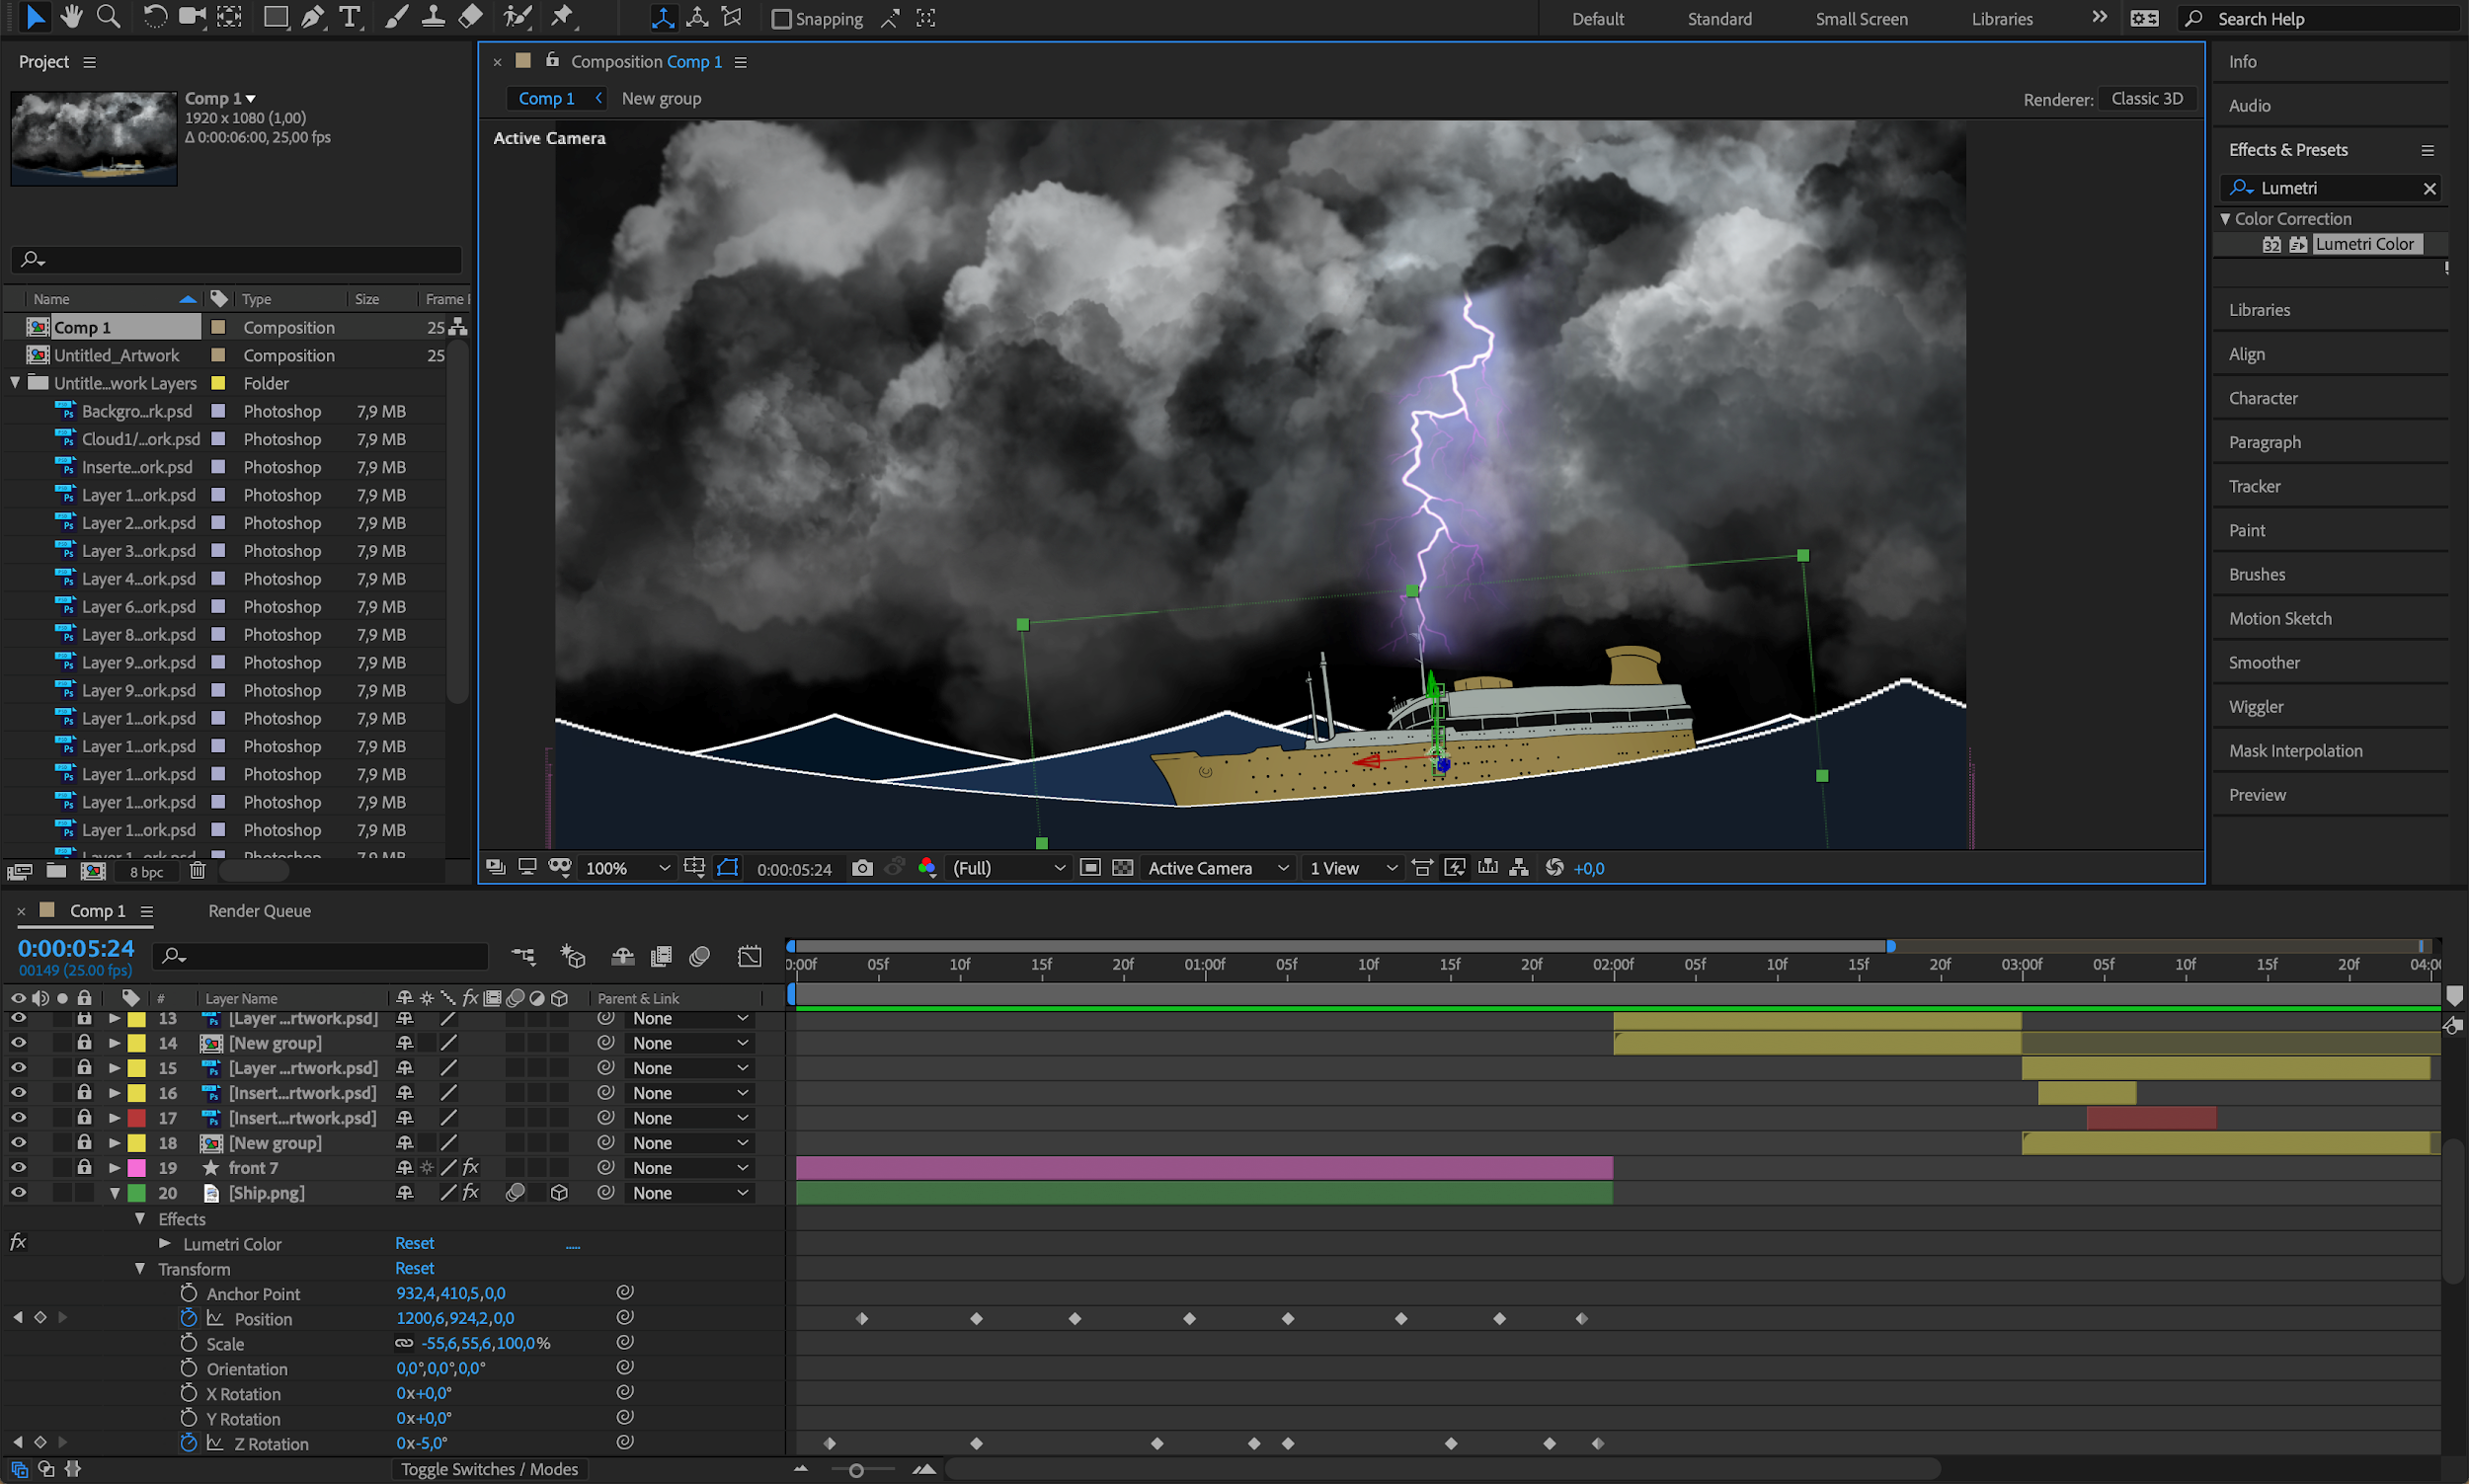
\includegraphics[width=0.5\textwidth]{../img/screenshot_aftereffects_intro.PNG}
\caption{Screenshot: After Effects Intro}
\label{fig:Screenshot: After Effects Intro}
\end{figure}

\subsubsection{Animation des Logos}
Das Video endet, wie in vielen bekannten Videos, mit unserem Logo. Hierfür musste das Edwards Biotope Logo animiert werden. 
Zunächst einmal wurde die Grafik (links) von dem Text (rechts) separiert. Die Absicht war es, zuerst das Symbol animiert einzublenden. Im Anschluss taucht der Name „Edwards Biotope“ auf. Dieser Text wurde ebenso animiert. Zum Schluss werden beide Teile wieder zusammengefügt. Die Bildreihenfolge Abbildung \ref{fig:Screenshots Animations 1} stellt diese Logo Animation dar. 
\begin{figure}[h]
\centering
 \subfloat[Screenshot: Animation 1]{{
\includegraphics[width=2cm]{../img/logo_animation/1/screenshot_logo_1.PNG} }}
\qquad
 \subfloat[Screenshot: Animation 2]{{
\includegraphics[width=2cm]{../img/logo_animation/1/screenshot_logo_2.PNG} }}
\qquad
 \subfloat[Screenshot: Animation 3]{{
\includegraphics[width=2cm]{../img/logo_animation/1/screenshot_logo_3.PNG} }}
\qquad
 \subfloat[Screenshot: Animation 4]{{
\includegraphics[width=2cm]{../img/logo_animation/1/screenshot_logo_4.PNG} }}
\caption{Screenshots Animations 1}%
 \label{fig:Screenshots Animations 1}%
\end{figure}
Allerdings war das nicht sehr überzeugend. Daher wurde weiterhin experimentiert. So wurde das Logo mit dem Spielnamen nicht mehr separiert animiert, sondern von Anfang an zusammen. Der Bildablauf  Abbildung \ref{fig:Screenshots Animations 2} veranschaulicht diese Animation.

\begin{figure}[h]
\centering
 \subfloat[Screenshot: Animation 5]{{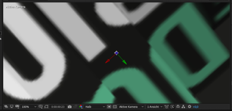
\includegraphics[width=2cm]{../img/logo_animation/2/screenshot_logo_5.PNG} }}
\qquad
 \subfloat[Screenshot: Animation 6]{{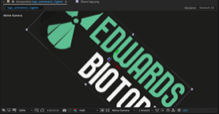
\includegraphics[width=2cm]{../img/logo_animation/2/screenshot_logo_6.PNG} }}
\qquad
 \subfloat[Screenshot: Animation 7]{{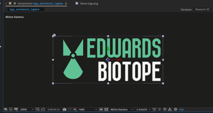
\includegraphics[width=2cm]{../img/logo_animation/2/screenshot_logo_7.PNG} }}
\caption{Screenshots Animations 2}%
 \label{fig:Screenshots Animations 2}%
\end{figure}
Im Anschluss wurde ein CC Light Sweep Effekt hinzugefügt und dafür gesorgt, dass das Logo kurz glänzt. Mit der Bestimmung der Richtung verläuft dieser Effekt von links oben nach rechts unten. Dieser Effekt ist auf der Abbildung \ref{fig:Screenshots Animations 3} zu sehen.

\begin{figure}[h]
\centering
 \subfloat[Screenshot: Animation 8]{{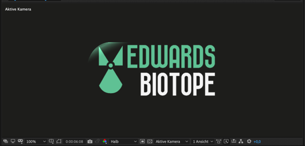
\includegraphics[width=2cm]{../img/logo_animation/3/screenshot_logo_8.PNG} }}
\qquad
 \subfloat[Screenshot: Animation 9]{{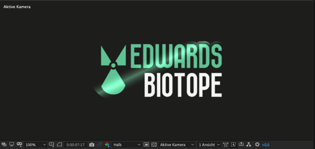
\includegraphics[width=2cm]{../img/logo_animation/3/screenshot_logo_9.PNG} }}
\qquad
 \subfloat[Screenshot: Animation 10]{{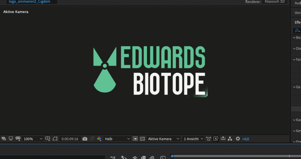
\includegraphics[width=2cm]{../img/logo_animation/3/screenshot_logo_10.PNG} }}
\caption{Screenshots Animations 3}%
 \label{fig:Screenshots Animations 3}%
\end{figure}

\subsubsection{Kompression des Trailers}
Das Endprodukt des Trailers war eine 8GB unkomprimierte AVI Video-Datei. In dieser Größe konnte es nicht auf den Server der Hochschule hochgeladen werden. Deshalb musste der Trailer noch komprimiert werden. Die Komprimierung erfolgte mit dem Adobe Media Encoder. Als Dateiformat wurde MOV ausgewählt. MOV hat den Vorteil, die Datenmenge mit verlustfreier und verlustbehaftender Komprimierung auf 70 MB zu verringern ohne sichtbare Qualitätsverluste zu liefern.
Die Animation befindet sich entsprechend im Anhang unter Logoanimation.


\subsection{Illustrationen}
Da dieses Kartenspiel stark im Einklang mit der dahinter stehenden Geschichte und der umgebenden Atmosphäre funktioniert, hatte die Fertigstellung der restlichen Kartenillustrationen hohe Priorität. Die Kolorierung sowie die Licht- und Schattengebung der ausstehenden Illustrationen brachten schließlich 46 individuelle Kartenmotive hervor.

\subsubsection{Lichtgebung und Schattierung}
Wie auch im letzten Semester gehörte das Setzen von Licht und Schatten zum letzten Schritt des Illustrationsdurchlaufes, welcher mit der Absicht der Erhaltung eines einheitlichen Illustrationsstiles erstellt wurde. Dabei unterteilte sich diese Aufgabe in die Nachbesserung der eingesetzten Farben innerhalb der geschlossenen Bereiche der Illustrationen sowie der eigentlichen Setzung von Schatten und Licht. Für diese Tätigkeiten wurde das Programm Procreate verwendet.

\subsubsection{Karten kolorieren}
Im 5. Semester der Projektarbeit wurden noch nicht alle Karten koloriert. Es waren noch 35 Karten, die keine Farbgebung erhalten haben. Die Kolorierung der Karten erfolgte auf einem MacBook Pro, mit der Software Adobe Photoshop CC 2019 und einem Grafiktablett von Bamboo. Um das einheitliche Gesamtbild sicherzustellen, wurden die Farben aus der Farbtabelle aus dem 5. Semester ausgewählt. Bei der Kolorierung wurde darauf geachtet, dass jede Karten einen ausgewogenen Komplementärkontrast hat. Zusätzlich benötigt jede Illustration mindestens drei Farben. Die Figuren müssen sich auch sichtbar von dem Hintergrund abheben. 
Entsprechende Materialien finden sich im Anhang unter "Karten\_Kolorieren".

\subsubsection{Spielkarten Outlines}
Um die Outlines aller Illustrationen herzustellen wurde Adobe Photoshop verwendet. Die vorher angefertigten Skizzen von Pamela Schättin und Daniel Scharrer, wurden gescannt und als Vorlage zur digitalen Ausarbeitung benutzt. Mit einem Canvasformat von 850 x 560 px wurde mit einer Linienstärke von 4 px die vorher positionierte Vorlage digital nachgezeichnet. Kleinere Änderungen bzw. Verbesserungen wurden dabei vorgenommen. Die Datei konnte nun als .psd-Datei abgespeichert werden und dem nächsten Prozess, also dem Colorblocking, zur Verfügung gestellt werden.

\subsubsection{Spielkartenrückseite Assets}
Da im Spiel auch Spielkarten verdeckt liegen sollen, sprich im Kartendeckstapel oder die Handkarten des Gegners, müssen auch Assets für die Rückseite einer Karte vorliegen. Um die Assets herzustellen wurde Adobe Photoshop verwendet. Diese soll visuell eindeutig und schnell erkennbar sein, da viele verschiedene bunte Farben auf der Kartenvorderseite (also Illustrationen) benutzt wurden. Um die Kartenrückseite davon abzuheben wurden wenige Farben und große Flächen benutzt. Zusätzlich wurde das Logo genutzt um eine eindeutige Zuweisung unserer IP herzustellen.

\subsubsection{Spielkarten Hintergründe}
Um die Hintergrüde aller Illustrationen herzustellen wurde Adobe Photoshop verwendet. Farblich wurde sich an der vorher festgelegt Farbpalette gehalten. Die vorher angefertigten Illustrationen (mit Outline, Colorblocking, Highlights und Shading) sind soweit fertig. Diese besitzen allerdings noch kein Hintergrund. Um diese Kreaturen, Quartiere und Phänomene nun noch in eine passende Umgebung zu versetzen, muss eine passende Unterwasserwelt her. Diese stellt in der Dimensionalen Wahrnehmung die hinterste Ebene dar. Das sich das Objekt(Kreatur, Quartier, Phänomen) visuell noch viel mehr vom Hintergrund absetzt, wurde zum Hintergrund ein minimalistischer Zeichenstil genutz(also ohne Outlines). Kleine kreative Spielereien, um die Spielkarten individueller zu machen, wurden hinzugefügt. Die fertige Illustration steht.

\subsubsection{Karten exportieren}
In Adobe InDesign musste der Rahmen der verschiedenen Kartentypen, mit den Kartenillustrationen und dem Kartennamen aus einer CSV Datei zusammengefügt werden. 
Der Rahmen musste noch einmal überarbeitet werden, da keine Effekte mehr auf der Karte ausgezeichnet werden. Deshalb wurde das Textfeld für die Effekte aus dem Rahmen mit Photoshop entfernt. Nach der Zusammenführung InDesign, entsteht ein PDF, aus diesem wurde mit dem Adobe Acrobat Reader Pro einzelne PNGs exportiert. Die Benennung der einzelnen Karten erfolgte aufgrund einer ID, so lässt sich die Karten im Sourcecode durch die ID zusammenführen.
Entsprechende Materialien finden sich im Anhang unter "Zusammenführung".

\subsubsection{Hauptmenü-Bildschirm Assets}
Um nicht direkt nachdem das Spiel gestartet wird in den Duell-Bildschirm zu kommen, wurde sich noch ein Hauptmenü-Bildschirm überlegt. Robert Sabo und Pamela Schättin kümmerten sich um die jeweiligen Assets die der Hauptmenü-Bildschirm beinhalten soll. Um die Assets herzustellen wurde Adobe Photoshop verwendet. Um einheitlich zu wirken, wurde der Illustrationsstil der Spielkarten hergenommen. Farblich wurde sich an der vorher festgelegt Farbpalette gehalten. Die Assets spiegeln das Spieluniversum, nämlich die Unterwasserwelt, visuell wieder. Es soll das Spieluniversum "Edwards Biotope" leicht "anteasern", und einen gewissen Eindruck des Spiels vermitteln. Das Background-Asset wurde von Robert Sabo entworfen und zeigt die Unterwasserwelt aus einem U-Boot heraus. links oben ist das Logo des Spiels zu sehen. Die Buttons wurden von Pamela Schättin erstellt. Die Buttons "Duell starten", "Deckeditor" und "Einstellungen" haben jeweils immer ein passendes Icon aus der Unterwasserwelt. Ausgegraute Buttons sollen noch nicht auswählbar und "klickbar" sein.

\subsubsection{Duell-Bildschrim-Assets}
Robert Sabo kümmerte sich um die jeweiligen Assets die der Duell-Bildschirm beinhalten soll. Um die Assets herzustellen wurde Adobe Photoshop verwendet. Um einheitlich zu wirken, wurde der Illustrationsstil der Spielkarten hergenommen. Farblich wurde sich an der vorher festgelegt Farbpalette gehalten. Die Assets spiegeln das Spieluniversum, nämlich die Unterwasserwelt, visuell wieder. Dabei ergibt sich eine gewisse Stimmung, die erreicht werden soll. Der Aufbau des Duell-Screens ist durch Skizzen und aus dem vorher angefertigten analogen und digitalen Prototyp entstanden. 
Nun zum Interface Design. Grade bei so einer komplexen Spielmechanik, ist es wichtig, das der User visuelle Eindrücke der gleichen Funktion zuordnen kann. Hierbei wurden viele grundlegende Gestaltungsgesetze für Interfaces beachtet und angewendet (Gesetz der Nähe, Gesetz der Gleichheit, Gesetz der Konstanz,...). Es soll auf dem Spielfeld klar ersichtlich sein, wo die Spielkarten abgelegt werden können, wo sich die jeweiligen Spielkartentypen wie z.B. Quartiere befinden, wo sich sowohl mein Deck, Friedhof und Handkarten, sowie die des Gegners befinden. Aber auch Interaktionsmöglichkeiten sollen auch auf dem ersten Blick ersichtlich sein. Dabei ist es wichtig das Spielfeld visuell von den Interaktionsmöglichkeiten wie Buttons und Anzeigefelder zu trennen. Das ist mit einem drei Spaltensystem gelöst worden. Die linke Spalte gibt Informationen über "Wer ist an der Reihe", einen Interaktionshinweis der Buttons und welche Karte ausgewählt ist wieder. Die rechte Spalte zeigt alle Buttons an, die mit dem Spielfeld interagieren und diese auch manipulieren können. Und die mittlere Spalte zeigt das tatsächliche Spielfeld, wo das Duell stattfindet, an. Um ein passendes Asset herzustellen müssen auch noch kommende Prozesse berücksichtigt werden. Sprich wie können diese Assets mit Hilfe der von IntelliJ IDEA vorhandenen Manipulationen, animiert werden. Rotieren, Skalieren, die Opacity ändern, Geschwindigkeit animieren etc. können später angewendet werden, um einen gewissen Interaktionsfeedback zu bekommen.




\pagebreak

\pagebreak
\begin{thebibliography}{9}
\bibitem{After Effects Einsteigertutorial}
After Effects Einsteigertutorial,
\url{https://www.youtube.com/watch?v=wrKdozeXA2Ul},
01.06.2019
\bibitem{How to Create Cartoon Animation}
How to Create Cartoon Animation,
\url{https://www.youtube.com/watch?v=QQgmXARn8aA},
01.06.2019
\bibitem{After Effects Tutorial: Logo Animations}
After Effects Tutorial: Logo Animations,
\url{https://www.youtube.com/watch?v=5WnaT1oFjt8},
01.06.2019
\bibitem{Shine Logo Animation in After Effects}
Shine Logo Animation in After Effects,
\url{https://www.youtube.com/watch?v=uEO_nLnytp0},
01.06.2019
\bibitem{Meld}
Tool: Meld
\url{https://meldmerge.org},
06.08.2019
\bibitem{Pairprogramming}
Improving Code Quality with Pair Programming, Ben Linders
\url{https://www.benlinders.com/2011/improving-code-quality-with-pair-programming/},
06.08.2019
\bibitem{Design Patterns}
Design Patterns,
Erich Gamma, Richard Helm, Ralph Johnson, John Vlissides
Verlag: mitp
ISBN: 978-3-8266-9700-5
1. Auflage 2015
\bibitem{PMD}
PMD - an extensible cross-language static code analyzer
\url{https://pmd.github.io}
06.08.2019
\bibitem{Metrics}
MetricsReloaded - automated code metrics plugin for IntelliJ IDEA
\url{https://github.com/BasLeijdekkers/MetricsReloaded}
06.08.2019
\end{thebibliography}

\listoffigures
\end{onehalfspace}
\end{document}